% Options for packages loaded elsewhere
\PassOptionsToPackage{unicode}{hyperref}
\PassOptionsToPackage{hyphens}{url}
%
\documentclass[
  man,floatsintext]{apa6}
\usepackage{amsmath,amssymb}
\usepackage{iftex}
\ifPDFTeX
  \usepackage[T1]{fontenc}
  \usepackage[utf8]{inputenc}
  \usepackage{textcomp} % provide euro and other symbols
\else % if luatex or xetex
  \usepackage{unicode-math} % this also loads fontspec
  \defaultfontfeatures{Scale=MatchLowercase}
  \defaultfontfeatures[\rmfamily]{Ligatures=TeX,Scale=1}
\fi
\usepackage{lmodern}
\ifPDFTeX\else
  % xetex/luatex font selection
\fi
% Use upquote if available, for straight quotes in verbatim environments
\IfFileExists{upquote.sty}{\usepackage{upquote}}{}
\IfFileExists{microtype.sty}{% use microtype if available
  \usepackage[]{microtype}
  \UseMicrotypeSet[protrusion]{basicmath} % disable protrusion for tt fonts
}{}
\makeatletter
\@ifundefined{KOMAClassName}{% if non-KOMA class
  \IfFileExists{parskip.sty}{%
    \usepackage{parskip}
  }{% else
    \setlength{\parindent}{0pt}
    \setlength{\parskip}{6pt plus 2pt minus 1pt}}
}{% if KOMA class
  \KOMAoptions{parskip=half}}
\makeatother
\usepackage{xcolor}
\usepackage{graphicx}
\makeatletter
\def\maxwidth{\ifdim\Gin@nat@width>\linewidth\linewidth\else\Gin@nat@width\fi}
\def\maxheight{\ifdim\Gin@nat@height>\textheight\textheight\else\Gin@nat@height\fi}
\makeatother
% Scale images if necessary, so that they will not overflow the page
% margins by default, and it is still possible to overwrite the defaults
% using explicit options in \includegraphics[width, height, ...]{}
\setkeys{Gin}{width=\maxwidth,height=\maxheight,keepaspectratio}
% Set default figure placement to htbp
\makeatletter
\def\fps@figure{htbp}
\makeatother
\setlength{\emergencystretch}{3em} % prevent overfull lines
\providecommand{\tightlist}{%
  \setlength{\itemsep}{0pt}\setlength{\parskip}{0pt}}
\setcounter{secnumdepth}{-\maxdimen} % remove section numbering
% Make \paragraph and \subparagraph free-standing
\ifx\paragraph\undefined\else
  \let\oldparagraph\paragraph
  \renewcommand{\paragraph}[1]{\oldparagraph{#1}\mbox{}}
\fi
\ifx\subparagraph\undefined\else
  \let\oldsubparagraph\subparagraph
  \renewcommand{\subparagraph}[1]{\oldsubparagraph{#1}\mbox{}}
\fi
% definitions for citeproc citations
\NewDocumentCommand\citeproctext{}{}
\NewDocumentCommand\citeproc{mm}{%
  \begingroup\def\citeproctext{#2}\cite{#1}\endgroup}
\makeatletter
 % allow citations to break across lines
 \let\@cite@ofmt\@firstofone
 % avoid brackets around text for \cite:
 \def\@biblabel#1{}
 \def\@cite#1#2{{#1\if@tempswa , #2\fi}}
\makeatother
\newlength{\cslhangindent}
\setlength{\cslhangindent}{1.5em}
\newlength{\csllabelwidth}
\setlength{\csllabelwidth}{3em}
\newenvironment{CSLReferences}[2] % #1 hanging-indent, #2 entry-spacing
 {\begin{list}{}{%
  \setlength{\itemindent}{0pt}
  \setlength{\leftmargin}{0pt}
  \setlength{\parsep}{0pt}
  % turn on hanging indent if param 1 is 1
  \ifodd #1
   \setlength{\leftmargin}{\cslhangindent}
   \setlength{\itemindent}{-1\cslhangindent}
  \fi
  % set entry spacing
  \setlength{\itemsep}{#2\baselineskip}}}
 {\end{list}}
\usepackage{calc}
\newcommand{\CSLBlock}[1]{\hfill\break\parbox[t]{\linewidth}{\strut\ignorespaces#1\strut}}
\newcommand{\CSLLeftMargin}[1]{\parbox[t]{\csllabelwidth}{\strut#1\strut}}
\newcommand{\CSLRightInline}[1]{\parbox[t]{\linewidth - \csllabelwidth}{\strut#1\strut}}
\newcommand{\CSLIndent}[1]{\hspace{\cslhangindent}#1}
\ifLuaTeX
\usepackage[bidi=basic]{babel}
\else
\usepackage[bidi=default]{babel}
\fi
\babelprovide[main,import]{english}
% get rid of language-specific shorthands (see #6817):
\let\LanguageShortHands\languageshorthands
\def\languageshorthands#1{}
% Manuscript styling
\usepackage{upgreek}
\captionsetup{font=singlespacing,justification=justified}

% Table formatting
\usepackage{longtable}
\usepackage{lscape}
% \usepackage[counterclockwise]{rotating}   % Landscape page setup for large tables
\usepackage{multirow}		% Table styling
\usepackage{tabularx}		% Control Column width
\usepackage[flushleft]{threeparttable}	% Allows for three part tables with a specified notes section
\usepackage{threeparttablex}            % Lets threeparttable work with longtable

% Create new environments so endfloat can handle them
% \newenvironment{ltable}
%   {\begin{landscape}\centering\begin{threeparttable}}
%   {\end{threeparttable}\end{landscape}}
\newenvironment{lltable}{\begin{landscape}\centering\begin{ThreePartTable}}{\end{ThreePartTable}\end{landscape}}

% Enables adjusting longtable caption width to table width
% Solution found at http://golatex.de/longtable-mit-caption-so-breit-wie-die-tabelle-t15767.html
\makeatletter
\newcommand\LastLTentrywidth{1em}
\newlength\longtablewidth
\setlength{\longtablewidth}{1in}
\newcommand{\getlongtablewidth}{\begingroup \ifcsname LT@\roman{LT@tables}\endcsname \global\longtablewidth=0pt \renewcommand{\LT@entry}[2]{\global\advance\longtablewidth by ##2\relax\gdef\LastLTentrywidth{##2}}\@nameuse{LT@\roman{LT@tables}} \fi \endgroup}

% \setlength{\parindent}{0.5in}
% \setlength{\parskip}{0pt plus 0pt minus 0pt}

% Overwrite redefinition of paragraph and subparagraph by the default LaTeX template
% See https://github.com/crsh/papaja/issues/292
\makeatletter
\renewcommand{\paragraph}{\@startsection{paragraph}{4}{\parindent}%
  {0\baselineskip \@plus 0.2ex \@minus 0.2ex}%
  {-1em}%
  {\normalfont\normalsize\bfseries\itshape\typesectitle}}

\renewcommand{\subparagraph}[1]{\@startsection{subparagraph}{5}{1em}%
  {0\baselineskip \@plus 0.2ex \@minus 0.2ex}%
  {-\z@\relax}%
  {\normalfont\normalsize\itshape\hspace{\parindent}{#1}\textit{\addperi}}{\relax}}
\makeatother

\makeatletter
\usepackage{etoolbox}
\patchcmd{\maketitle}
  {\section{\normalfont\normalsize\abstractname}}
  {\section*{\normalfont\normalsize\abstractname}}
  {}{\typeout{Failed to patch abstract.}}
\patchcmd{\maketitle}
  {\section{\protect\normalfont{\@title}}}
  {\section*{\protect\normalfont{\@title}}}
  {}{\typeout{Failed to patch title.}}
\makeatother

\usepackage{xpatch}
\makeatletter
\xapptocmd\appendix
  {\xapptocmd\section
    {\addcontentsline{toc}{section}{\appendixname\ifoneappendix\else~\theappendix\fi\\: #1}}
    {}{\InnerPatchFailed}%
  }
{}{\PatchFailed}
\keywords{eye-tracking, online, webcam, jsPsych, cognitive science\newline\indent Word count: X}
\usepackage{lineno}

\linenumbers
\usepackage{csquotes}
\ifLuaTeX
  \usepackage{selnolig}  % disable illegal ligatures
\fi
\usepackage{bookmark}
\IfFileExists{xurl.sty}{\usepackage{xurl}}{} % add URL line breaks if available
\urlstyle{same}
\hypersetup{
  pdftitle={What paradigms can webcam eye-tracking be used for? Attempted replications of five ``classic'' cognitive science experiments},
  pdfauthor={Joshua R. de Leeuw1, Rachel Ryskin2, Ariel N. James3, Joshua K. Hartshorne4, Haylee Backs1, Nandeeta Bala1, Laila Barcenas-Meade1, Samata Bhattarai1, Tessa Charles1, Gerasimos Copoulos1, Claire Coss1, Alexander Eisert1, Elena Furuhashi1, Keara Ginell1, Anna Guttman-McCabe1, Emma (Chaz) Harrison1, Laura Hoban1, William A. Hwang1, Claire Iannetta1, Kristen M. Koenig1, Chauncey Lo1, Victoria Palone1, Gina Pepitone1, Margaret Ritzau1, Yi Hua Sung1, \& Lauren Thompson1},
  pdflang={en-EN},
  pdfkeywords={eye-tracking, online, webcam, jsPsych, cognitive science},
  hidelinks,
  pdfcreator={LaTeX via pandoc}}

\title{What paradigms can webcam eye-tracking be used for? Attempted replications of five ``classic'' cognitive science experiments}
\author{Joshua R. de Leeuw\textsuperscript{1}, Rachel Ryskin\textsuperscript{2}, Ariel N. James\textsuperscript{3}, Joshua K. Hartshorne\textsuperscript{4}, Haylee Backs\textsuperscript{1}, Nandeeta Bala\textsuperscript{1}, Laila Barcenas-Meade\textsuperscript{1}, Samata Bhattarai\textsuperscript{1}, Tessa Charles\textsuperscript{1}, Gerasimos Copoulos\textsuperscript{1}, Claire Coss\textsuperscript{1}, Alexander Eisert\textsuperscript{1}, Elena Furuhashi\textsuperscript{1}, Keara Ginell\textsuperscript{1}, Anna Guttman-McCabe\textsuperscript{1}, Emma (Chaz) Harrison\textsuperscript{1}, Laura Hoban\textsuperscript{1}, William A. Hwang\textsuperscript{1}, Claire Iannetta\textsuperscript{1}, Kristen M. Koenig\textsuperscript{1}, Chauncey Lo\textsuperscript{1}, Victoria Palone\textsuperscript{1}, Gina Pepitone\textsuperscript{1}, Margaret Ritzau\textsuperscript{1}, Yi Hua Sung\textsuperscript{1}, \& Lauren Thompson\textsuperscript{1}}
\date{}


\shorttitle{Webcam eye-tracking paradigms}

\authornote{

The authors made the following contributions. Joshua R. de Leeuw: Conceptualization, Data curation, Formal analysis, Investigation, Methodology, Project administration, Software, Supervision, Validation, Visualization, Writing - original draft, Writing - review \& editing; Rachel Ryskin: Conceptualization, Formal analysis, Visualization, Writing - original draft, Writing - review \& editing; Ariel N. James: Conceptualization, Formal analysis, Visualization, Writing - original draft, Writing - review \& editing; Joshua K. Hartshorne: Conceptualization, Formal analysis, Visualization, Writing - original draft, Writing - review \& editing; Haylee Backs: Investigation, Methodology, Software; Nandeeta Bala: Investigation, Methodology, Software; Laila Barcenas-Meade: Investigation, Methodology, Software; Samata Bhattarai: Investigation, Methodology, Software; Tessa Charles: Investigation, Methodology, Software; Gerasimos Copoulos: Investigation, Methodology, Software; Claire Coss: Investigation, Methodology, Software; Alexander Eisert: Investigation, Methodology, Software; Elena Furuhashi: Investigation, Methodology, Software; Keara Ginell: Investigation, Methodology, Software; Anna Guttman-McCabe: Investigation, Methodology, Software; Emma (Chaz) Harrison: Investigation, Methodology, Software; Laura Hoban: Investigation, Methodology, Software; William A. Hwang: Investigation, Methodology, Software; Claire Iannetta: Investigation, Methodology, Software; Kristen M. Koenig: Investigation, Methodology, Software; Chauncey Lo: Investigation, Methodology, Software; Victoria Palone: Investigation, Methodology, Software; Gina Pepitone: Investigation, Methodology, Software; Margaret Ritzau: Investigation, Methodology, Software; Yi Hua Sung: Investigation, Methodology, Software; Lauren Thompson: Investigation, Methodology, Software.

Correspondence concerning this article should be addressed to Joshua R. de Leeuw, 124 Raymond Ave, Poughkeepsie, NY 12604, USA. E-mail: \href{mailto:jdeleeuw@vassar.edu}{\nolinkurl{jdeleeuw@vassar.edu}}

}

\affiliation{\vspace{0.5cm}\textsuperscript{1} Cognitive Science Department, Vassar College\\\textsuperscript{2} Department of Cognitive \& Information Science, University of California, Merced\\\textsuperscript{3} Psychology Department, Macalester College\\\textsuperscript{4} Department of Psychology \& Neuroscience, Boston College}

\abstract{%
We tested whether the results of five different eye-tracking experiments in the cognitive psychology literature would replicate in a webcam-based eye-tracking format. Specifically, we carried out five experiments by integrating two javascript-based tools: js.psych and a modified version of Webgazer.js. In order to represent a wide range of applications of eye-tracking to cognitive psychology, we chose two psycholinguistic experiments, two memory experiments, and a decision-making experiment. These studies also varied in the type of eye-tracking display, including screens split into halves (Exps. 3 and 5) or quadrants (Exps. 2 \& 4), or composed scenes with regions of interest that varied in size (Exp. 1). Outcomes were mixed. The least successful replication attempt was Exp. 1; we did not obtain a condition effect in our remote sample (1a), nor in an in-lab follow-up (1b). However, the other four experiments were more successful, replicating a blank-screen effect (Exp. 2), a novelty preference (Exp. 3), a verb bias effect (Exp. 4), and a gaze-bias effect in decision-making. These results suggest that webcam-based eye tracking can be used to detect a variety of cognitive phenomena, including those with sensitive time, although paradigms that require high spatial resolution should be adapted to coarser quadrant or split-half displays.
}



\begin{document}
\maketitle

The use of eye-tracking to study cognition took off when Alfred Yarbus used suction cups to affix a mirror system to the sclera of the eye in order to monitor eye position during the perception of images (Yarbus, 1967). In one study, participants viewed a painting depicting multiple people in a complex interaction inside of a 19th century Russian home. Yarbus showed, among other things, that the scan paths and locations of fixations were largely dependent on the instructions given to participants (e.g., View the picture freely vs.~Remember the position of the people and objects in the room). In other words, the cognitive processing that the individual is engaged in drives the visuo-motor system. Since these findings, eye-tracking has become a central method in cognitive science research Rayner (1998). For example, gaze location during natural scene perception is used to test theories of visual attention (e.g., Henderson \& Hayes, 2017), and eye-movements during auditory language comprehension, using the ``visual world paradigm,'' demonstrated the context-dependent and incremental nature of language processing (e.g., Tanenhaus, Spivey-Knowlton, Eberhard, \& Sedivy, 1995).

An important limitation of the eye-tracking methodology is that it has typically required costly equipment (eye-trackers can range in price from a few thousand dollars to tens of thousands of dollars), particular laboratory conditions (a quiet room with consistent indoor lighting conditions), and a substantial time investment (e.g., bringing participants into a laboratory one at a time). This limits who can conduct eye-tracking research -- not all researchers have the necessary resources -- and who can participate in eye-tracking research. Most eye-tracking study participants are from western, educated, industrialized, rich, and democratic {[}WEIRD; Henrich, Heine, and Norenzayan (2010){]} convenience samples (but see Ryskin, Salinas, Piantadosi, \& Gibson, 2023), which diminishes the generalizability of the findings and the scope of conclusions that can be drawn about human cognition.

Advances in software for online data collection (de Leeuw, 2015; Papoutsaki et al., 2016) have the potential to address this shortcoming by expanding access to eye-tracking technology for researchers and making it feasible to broaden and diversify the participant samples. In particular, \texttt{Webgazer.js} (Papoutsaki et al., 2016) is a webcam-based Javascript plug-in that works in the browser. It can be integrated with any Javascript web interface. As a result, it can be used in conjunction with many existing platforms for online behavioral data collection that are familiar to cognitive scientists, such as \texttt{jsPsych} (de Leeuw, 2015), \texttt{Gorilla} (Anwyl-Irvine, Massonnié, Flitton, Kirkham, \& Evershed, 2020), or \texttt{lab.js} (Henninger, Shevchenko, Mertens, Kieslich, \& Hilbig, 2021). However, the added convenience comes at the cost of spatial and temporal resolution. The extent of this loss of precision and its impact on the kinds of research questions that webcam eye-tracking is appropriate for are the subject of the current study.

A few previous studies have used webcam eye-tracking in the context of behavioral/cognitive science experiments and reported on the quality of the data. In what follows, we provide a brief review of the published work that we are aware of (note that we focus on studies with adult participants as the considerations for eye-tracking of children are substantially different, but see e.g., Bánki, Eccher, Falschlehner, Hoehl, \& Markova, 2022).

Semmelmann and Weigelt (2018) compared eye-tracking results between in-lab (n=29) and online (n=28) studies in three tasks: fixation, pursuit, and free viewing. They used the \texttt{Webgazer.js} library (Papoutsaki et al., 2016) and programmed tasks in HTML/Javascript directly. The first two tasks tested measurement of basic gaze properties. In the fixation task, participants were asked to fixate a dot, and in the pursuit task, they were asked to follow a dot with their eyes. In the free viewing task, the eye movements may have been more semantically driven: participants were shown a picture of a human face and asked to look wherever they wanted to on the image. Webgazer was successful in accurately detecting fixation locations and saccades in all three tasks, though online data (collected through a crowdsourcing platform) were slightly more variable and delayed relative to the in-lab data. The free viewing task replicated previously observed statistical patterns (e.g., more fixations on eyes than mouths).

Similarly, Yang and Krajbich (2021) used the \texttt{Webgazer.js} library (Papoutsaki et al., 2016) combined with the \texttt{jsPsych} library for conducting behavioral experiments in a web browser (de Leeuw, 2015), to replicate a well-established link between value-based decision-making and eye gaze Krajbich, Armel, \& Rangel (2010). Online participants (n=38) first saw a series of images of 70 snack foods and rated how much they liked each one. During the primary task, on each of 100 trials, two of the snack food images were displayed on the left and right sides of the display and participants chose the one that they preferred while their gaze was monitored. As in previous work, participants were biased to choose the option they had spent more time looking at. The authors also implemented a code modification to address temporal delays in \texttt{WebGazer}.

Several papers have used the \texttt{WebGazer.js} library (via different interfaces) to replicate visual world paradigm studies. Slim and Hartsuiker (2022) used the \texttt{PCIbex} online experiment platform (Zehr \& Schwarz, 2018) to replicate a study in which participants (n=90) listened to sentences (e.g., Mary reads a letter) while viewing four pictures displayed across the four quadrants of the screen {[}e.g., a letter, a backpack, a car and a wheelchair; Dijkgraaf, Hartsuiker, and Duyck (2017){]}. When the verb in the sentence was \emph{constraining} (e.g., read) with respect to the display (only the letter would be an appropriate continuation), listeners made more fixations to the target image (letter) than when the verb was \emph{neutral} (e.g., Mary steals a letter), as in previous work. However, they observed a substantial delay of \textasciitilde200ms in the onset of the effect relative to the in-lab study with an infrared eyetracker and a reduction in effect size (despite a threefold increase in sample size relative to the original). The authors noted that delay was particularly problematic given that the purpose of the original study was to capture aspects of predictive or anticipatory processing: in the original study, but not in the web replication, the difference between \emph{constraining} and \emph{neutral} conditions emerged before the onset of the final noun (e.g., letter). Similarly, Degen, Kursat, and Leigh (2021) reported that effects of scalar implicature processing (comparing looks to the target in a four quadrant display for sentences such as ``Click on the girl that has \emph{some} apples'' vs.~``Click on the girl that has \emph{three} apples'' ) were smaller and delayed relative to those observed in the lab (Sun \& Breheny, 2020).

In contrast, using the \texttt{Gorilla} experiment platform (Anwyl-Irvine et al., 2020), Prystauka, Altmann, and Rothman (2023) observed robust effects of verb semantics and lexical interference in similar time windows to previous in-lab studies (Altmann \& Kamide, 1999; Kukona, Cho, Magnuson, \& Tabor, 2014), though a direct comparison was not possible because their studies used different materials than the in-lab experiments they were conceptually replicating. Furthermore, using \texttt{jsPsych}, Vos, Minor, and Ramchand (2022) closely replicated the magnitude and timecourse of effects in a lab-based visual world paradigm where the regions of interest (ROIs) consisted of the left and right halves of the display, suggesting that the concerns about poor temporal resolution can be mitigated. Indeed, the eye-tracking plug-in in \texttt{jsPsych} uses a fork of \texttt{Webgazer.js} in which certain modifications have been made to minimize processing time. \footnote{See discussion at \url{https://github.com/jspsych/jsPsych/discussions/1892}}

Finally, Van der Cruyssen et al. (2023) used \texttt{WebGazer.js} in conjunction with \texttt{PsychoJS} to conceptually replicate three paradigms, one which is analogous to Yang and Krajbich (2021), another testing the novelty preference (tendency for learners to look more at an object that they have not yet studied), and a visual world paradigm study with 4 objects, similar to Prystauka et al. (2023). These replications were successful but they noted reductions in effect sizes relative to an in-lab dataset. They did not address whether there were temporal delays.

In sum, webcam eye-tracking has been used to varying degrees of success across a small set of paradigms that are used in cognitive science research. One configuration, \texttt{jsPsych} with a modification of \texttt{WebGazer.js}, appears to have circumvented initial limitations in temporal precision (Krajbich et al., 2010; Vos et al., 2022) but has only been tested with paradigms with minimal requirements in terms of spatial precision (both experiments used the two sides of the display as the ROIs). Further, the extent to which noise in the measurement is due to the software and hardware limitations as opposed to the difference between the in-lab and online settings remains unclear. In the current work, we evaluate a broad variety of paradigms in terms of their suitability for webcam eye-tracking in order to provide guidance for cognitive scientists aiming to increase and diversify participation in their eye-tracking-based research.

\section{Present work}\label{present-work}

In order to validate the online eye-tracking methodology, with the particular configuration known to have the greatest temporal precision, \texttt{jsPsych} and a modification of \texttt{Webgazer}, we set out to reproduce five previously published studies representing a variety of questions, topics, and paradigms. The goal was to examine the strengths and weaknesses of webcam eye-tracking for common paradigms in cognitive science, across a broad range of research areas.

\subsection{Selection of Studies}\label{selection-of-studies}

Studies with large effect sizes and which are known to replicate are ideal targets for further replication; otherwise, it can be difficult to distinguish a failure of the method from a failure of the original study to replicate. In practice, replications (successful or otherwise) have only been reported for a small number of studies, so we ultimately included some studies with unknown replicability. We addressed this in several ways. First, replicating five very different studies from different research traditions decreases our reliance on any one study. Second, we include several `'sanity check'' analyses, such as the correlation between calibration accuracy and effect size. If the effect is real but there is noise from low-accuracy eye-tracking, this correlation should be substantial. Third, for two of the studies, we had comparison data collected in-lab either using \texttt{jsPsych} or a more traditional eyetracker technology, allowing us to directly assess the impact of differences in subject population and equipment/setting.

We chose five high-impact eye-tracking studies involving adult subjects (for an investigation of WebGazer's validity for developmental research, see Steffan et al., 2024 for a comparison of remote WebGazer and in-lab anticipatory looking effects in 18-27-month-old participants). Our goal was to include experiments from a range of topic areas (e.g., memory, decision making, psycholinguistics) and paradigms (two halves of the screen, visual world paradigm with four quadrants, visual world paradigm with ``naturalistic'' scenes). As noted above, we had a preference for well-established findings that are known to replicate, though for sake of diversity this was not always possible. Table \ref{tab:studies-table} provides an overview of the five studies we selected.

\begin{table}[tbp]

\begin{center}
\begin{threeparttable}

\caption{\label{tab:studies-table}Studies selected for replication attempts. Citation counts based on Google Scholar (May 2024).}

\small{

\begin{tabular}{llll}
\toprule
Citation & \multicolumn{1}{c}{Topic Area} & \multicolumn{1}{c}{Paradigm} & \multicolumn{1}{c}{Citations}\\
\midrule
Altmann \& Kamide, 1999 & Psycholinguistics & Natural Scenes & 2,130\\
Johansson \& Johansson, 2014 & Memory & Four Quadrants & 259\\
Manns, Stark, \& Squire, 2000 & Memory & Two Halves & 134\\
Snedeker \& Trueswell, 2004 & Psycholinguistics & Four Quadrants & 487\\
Shimojo et al., 2003 & Decision Making & Two Halves & 1,146\\
\bottomrule
\end{tabular}

}

\end{threeparttable}
\end{center}

\end{table}

\section{General Methods}\label{general-methods}

\subsection{Participants}\label{participants}

Participants completed the experiment remotely and were recruited
through the Prolific platform. In order to have access to the
experiment, participants had to meet the following criteria: 18 years of
age or older, fluency in English, and access to a webcam. All
participants provided informed consent. The studies were approved by the
Vassar College Institutional Review Board.

In addition, an in-person replication was conducted for Experiment 1.
Information about the sample is given in the Experiment 1 Method sections.

In order to have adequate statistical power and precision, we aimed for
2.5x the sample size of the original experiment, following the heuristic
of Simonsohn (Simonsohn, 2015). In Experiment 5, the original sample size was so
small that we opted to collect 5x the number of participants to increase
precision. Because of budget and time constraints we were unable to
replace the data for subjects who were excluded or whose data was
missing due to technical failures.

\subsection{Equipment}\label{equipment}

We used a fork of the \texttt{webgazer.js} library for webcam eye-tracking
(Papoutsaki et al., 2016), implemented in \texttt{jsPsych}, a Javascript
library for running behavioral experiments in a web browser
(de Leeuw, 2015). Our fork included changes to
\texttt{webgazer.js} in order to improve data quality for experiments in which
the precise timing of stimulus onsets is relevant. Specifically, we
implemented a polling mode so that gaze predictions could be requested
at a regular interval, which improved the sampling rate considerably in
informal testing. This modification is similar to what Yang and Krajbich
(2021) reported improved the sampling rate in their study of
webgazer. We also adjusted the mechanism for recording time stamps of
each gaze prediction, so that the time stamp reported by webgazer is
based on when the video frame is received and not when the computation
of the gaze point is finished.

\subsection{Eye-tracking Calibration and Validation}\label{eye-tracking-calibration-and-validation}

When participants began the experiment, they were notified the webcam
would be used for eye tracking but no video would be saved. They were
asked to remove glasses if possible, close any other tabs or apps, turn
off notifications, and make sure their face was lit from the front. The
webcam's view of the participant popped up on the screen, and
participants were asked to center their face in the box and keep their
head still. The experiment window then expanded to full screen, and
participants began the eye-tracking calibration.

During the calibration, dots appeared on the screen one at a time in
different locations, and the participants had to fixate them and click
on each one. Once they clicked on a dot, it would disappear and a new
one would appear in a different location on the screen. The locations of
calibration dots were specific to each experiment (details below) and
appeared in the areas of the screen where the visual stimuli would
appear during the main task in order to ensure that eye movements were
accurately recorded in the relevant regions of interest. After the
calibration was completed, the validation began. Participants were asked
to go through the same steps as the calibration, except that they only
fixated the dots as they appeared in different locations on the screen.
If accuracy on the validation was too low (fewer than 50\% of looks
landed within a 200 px radius of the validation points),
participants were given an opportunity to re-start the calibration and
validation steps. If the second attempt also lead to low validation
accuracy, participants were informed that they could not participate in
the study.

\subsection{Pre-registration}\label{pre-registration}

These data were collected within the context of an undergraduate research methods course. Groups of students (co-authors) designed and programmed experiments in jsPsych, pre-registered their planned analyses, and collected data through Prolific under the supervision of the first author. The OSF repositories associated with these experiments are linked in the methods sections of each individual study. Note that in the current paper we expand on those pre-registered analyses (e.g., including analyses of the calibration quality). All analysis code underlying this paper can be found in the Github repository: \url{https://github.com/jodeleeuw/219-2021-eyetracking-analysis}

\subsection{Data pre-processing}\label{data-pre-processing}

We used R (Version 4.4.0; R Core Team, 2021) and the R-packages \emph{afex} (Version 1.3.1; Singmann, Bolker, Westfall, Aust, \& Ben-Shachar, 2021), \emph{broom.mixed} (Version 0.2.9.5; Bolker \& Robinson, 2020), \emph{dplyr} (Version 1.1.4; Wickham, François, Henry, \& Müller, 2021), \emph{forcats} (Version 1.0.0; Wickham, 2021a), \emph{ggplot2} (Version 3.5.1; Wickham, 2016), \emph{jsonlite} (Version 1.8.8; Ooms, 2014), \emph{lme4} (Version 1.1.35.3; Bates, Mächler, Bolker, \& Walker, 2015), \emph{lmerTest} (Version 3.1.3; Kuznetsova, Brockhoff, \& Christensen, 2017), \emph{Matrix} (Version 1.7.0; Bates \& Maechler, 2021), \emph{papaja} (Version 0.1.2; Aust \& Barth, 2020), \emph{readr} (Version 2.1.5; Wickham \& Hester, 2020), \emph{shiny} (Chang et al., 2021), \emph{stringr} (Version 1.5.1; Wickham, 2019), \emph{tidyr} (Version 1.3.1; Wickham, 2021b), and \emph{tinylabels} (Version 0.2.4; Barth, 2022) for all our analyses.

\section{Experiment 1}\label{experiment-1}

The first study was a replication attempt of
Altmann and Kamide (1999). Altmann and Kamide used the
visual world eye-tracking paradigm (Tanenhaus et al., 1995) to show that
meanings of verbs rapidly constrain the set of potential subsequent
referents in sentence processing. For example, when looking at the
display in Figure~\ref{fig:E1-example-trial} and listening to a sentence like
``The boy will eat the\ldots,'' participants are more likely to look at the cake than
when they hear ``The boy will move the\ldots,'' in which case they tend to look at the
train, presumably because cakes are edible and trains are not. Semantic
information available at the verb is used to anticipate upcoming
linguistic input.

We first collected data from participants via Prolific, then conducted a follow-up in-lab replication; both the remote and the in-lab replications used WebGazer and identical materials and procedures.

\subsection{Method}\label{method}

All stimuli, experiment scripts, data, analysis scripts, and a
pre-registration are available on the Open Science Framework at
\url{https://osf.io/s82kz}.

\subsubsection{Participants}\label{participants-1}

\paragraph{Remote sample}\label{remote-sample}

Sixty participants were paid \$2.60 for their participation. Our sample size
of participants was determined by the total run time of our experiment,
\textasciitilde10 minutes, and the allotted funding from the Vassar College Cognitive
Science Department. From this information, we calculated a reasonable
number of participants we could afford to compensate on Prolific. Note
that the sample size of the original study was 24. For unknown reasons,
2 of the subjects' results were not recorded, so in the analysis, we
worked with data collected from 58 participants.

\paragraph{In-lab sample}\label{in-lab-sample}

Forty-nine participants completed the study in a lab setting. They were recruited via the college subject pool. Participants needed to be 18 years of age or older and native speakers of English. The study was approved by the Institutional Review Board at Boston College.

\subsubsection{Procedure}\label{procedure}

The task began with a 9-point eye-tracker calibration
and validation (Figure~\ref{fig:E1-calibration-figure}).
During the experiment, the participants were
simultaneously presented with a visual image and a corresponding audio
recording of a spoken sentence. Participants had to input a keyboard
response indicating ``yes'' or ``no'' as to whether the sentence they heard
was feasible given the visual image. There were two practice trials to
ensure that participants understood the instructions
before they undertook the main portion of the experiment. Participants'
reaction times, keyboard responses, and looks to objects in the scene
were recorded for each trial.

\begin{verbatim}
## Warning: A numeric `legend.position` argument in `theme()` was deprecated in ggplot2
## 3.5.0.
## i Please use the `legend.position.inside` argument of `theme()` instead.
## This warning is displayed once every 8 hours.
## Call `lifecycle::last_lifecycle_warnings()` to see where this warning was
## generated.
\end{verbatim}

\begin{figure}
\centering
\includegraphics{manuscript_files/figure-latex/E1-calibration-figure-1.pdf}
\caption{\label{fig:E1-calibration-figure}Calibration and validation point locations for Experiment 1. Black points were used for calibration. Red crosses were used for checking the accuracy of the calibration.}
\end{figure}

\subsubsection{Materials \& Design}\label{materials-design}

The visual stimuli were created through Canva and depicted an agent
accompanied by four to five objects in the scene (see Figure~\ref{fig:E1-example-trial}). On
critical trials, participants heard one of two sentences associated with
the scene. In the restrictive condition, the sentence (e.g., ``The boy
will eat the cake'') contained a verb (e.g., ``eat'') which restricts the
set of possible subsequent referents (e.g., to edible things). Only the
target object (e.g., the cake) was semantically consistent with the
verb's meaning. In the non-restrictive condition, the sentence (e.g.,
``The boy will move the cake'') contained a verb (e.g., ``move'') which does
not restrict the set of possible subsequent referents. The target object
(e.g., the cake) as well as the distractor objects (e.g., the train, the
ball, etc.) were semantically consistent with the verb's meaning. Both
sentences were compatible with the scene, such that the correct keyboard
response for the critical trials was ``yes.'' Filler trials consisted of
scenes that also contained an agent surrounded by objects as in the critical trials, but corresponding sentences named an object that was not present in the scene. The correct keyboard response for the filler
trials was ``no.''

\begin{figure}
\centering
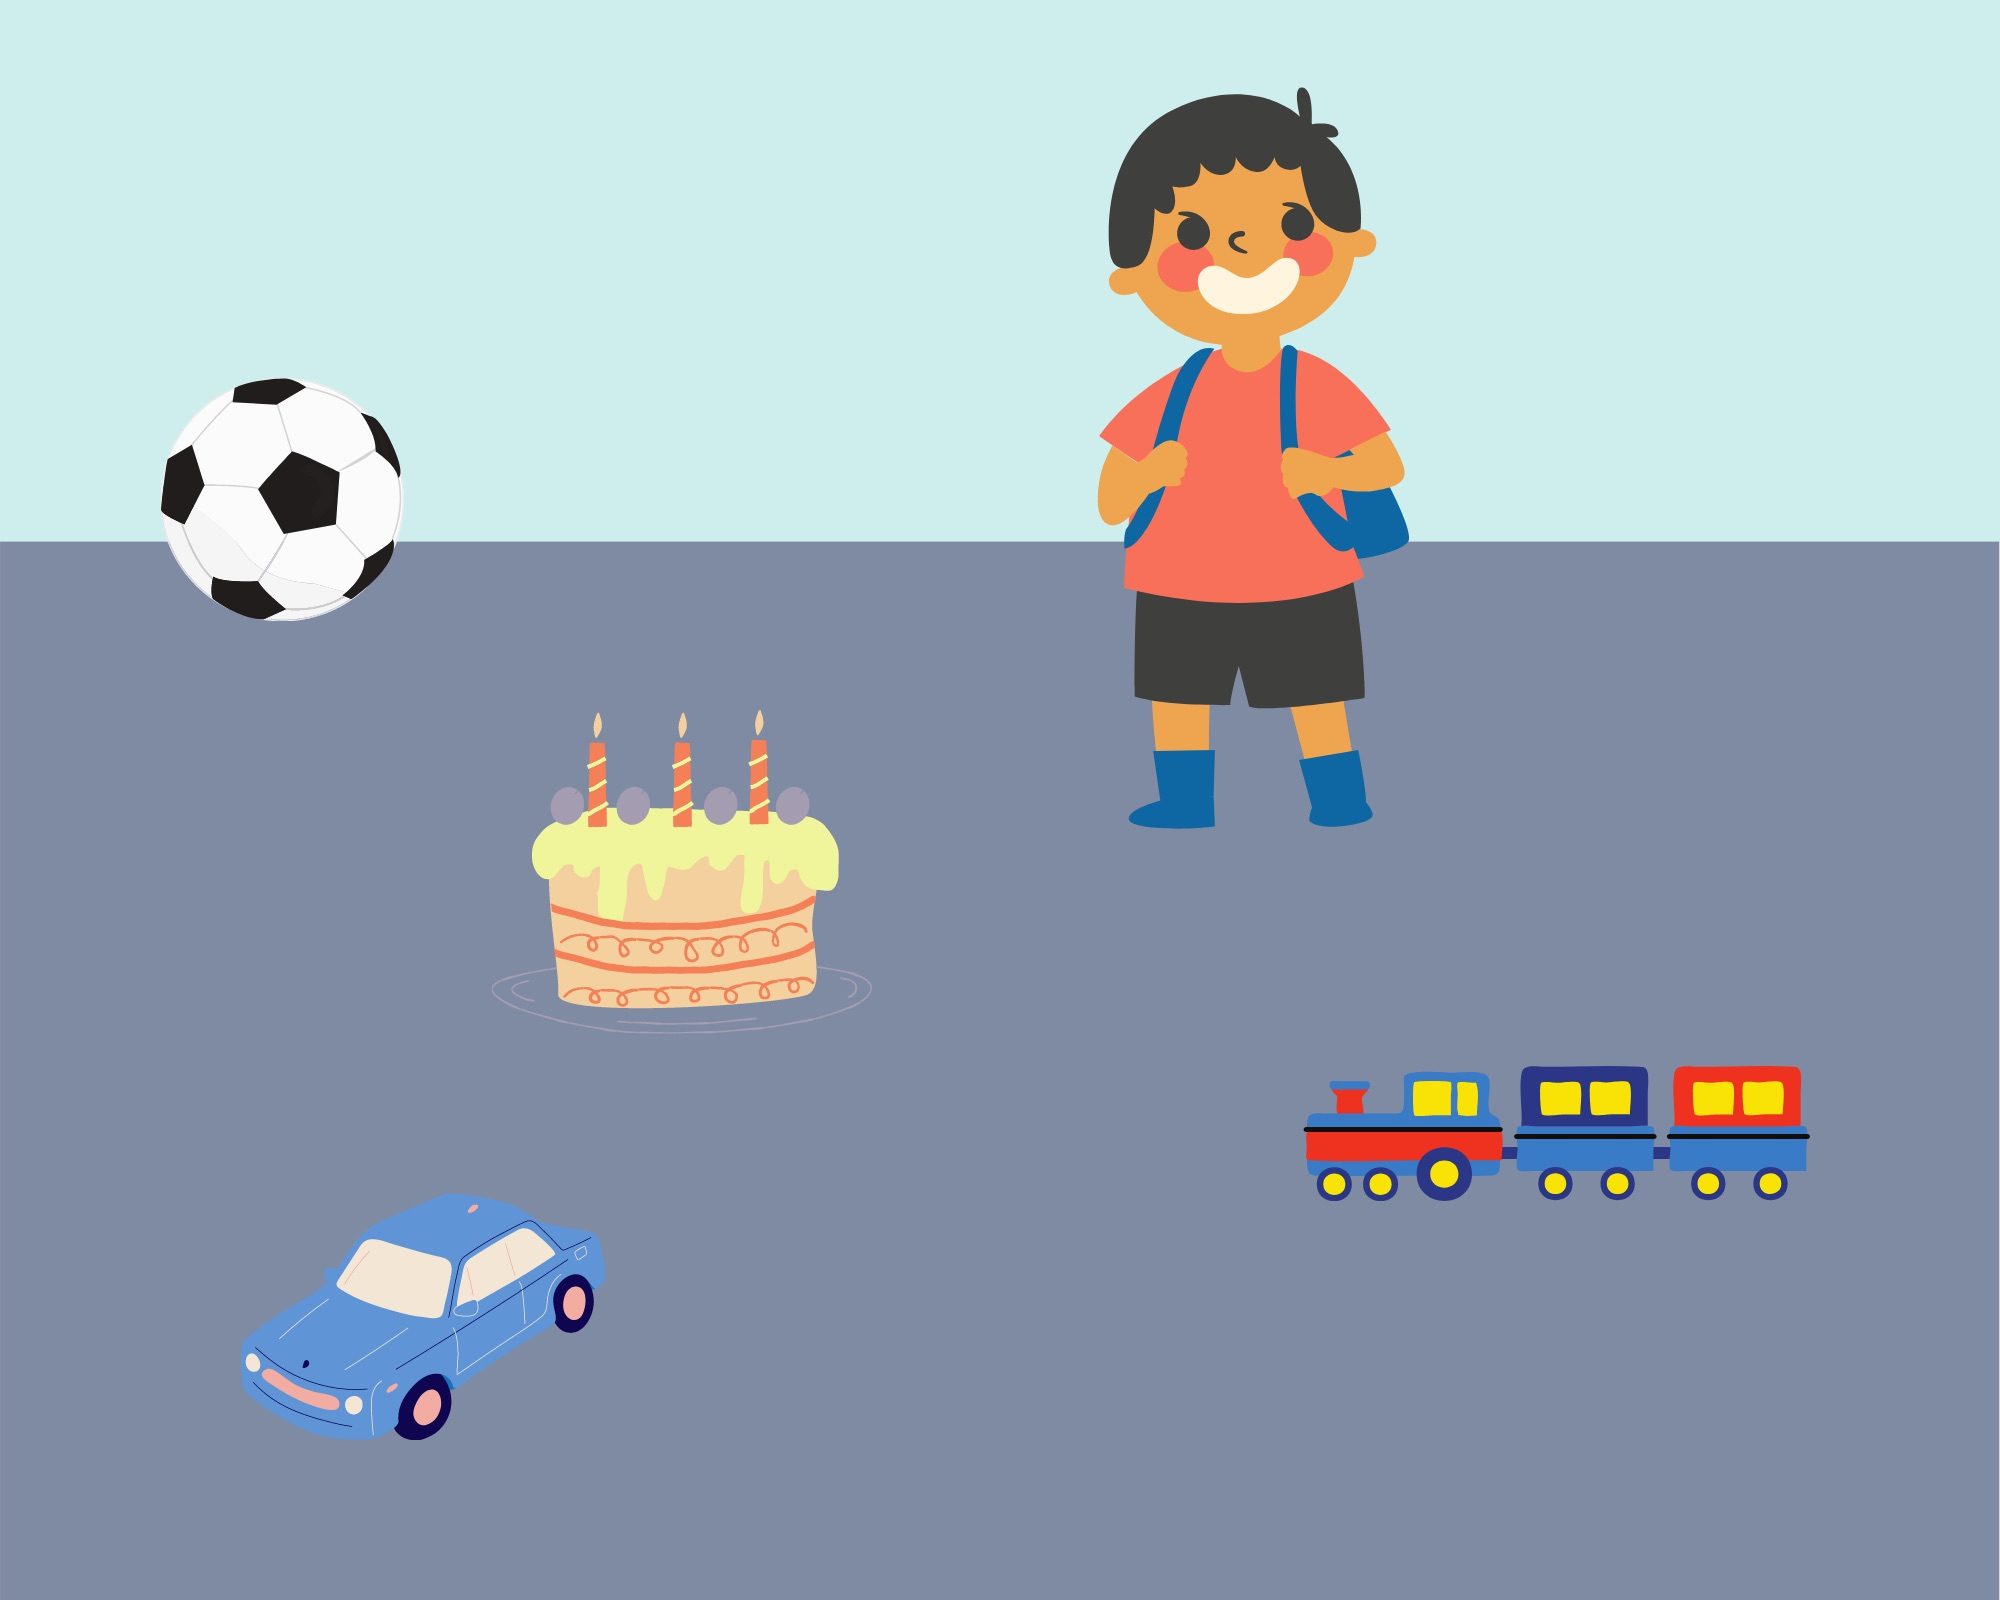
\includegraphics{group-a/E1-example-trial.jpeg}
\caption{\label{fig:E1-example-trial}Example trial from Experiment 1. Participants would hear a sentence (e.g., ``The boy will eat the cake'') and respond according to whether the sentence matched the picture.}
\end{figure}

Each participant was presented with sixteen critical trials (eight in
the restrictive condition, eight in the non-restrictive condition) and
sixteen fillers for a total of 32 trials. The order of trials and the
assignment of critical scene to condition was random on a
subject-by-subject basis.

\subsubsection{Data pre-processing and analysis}\label{data-pre-processing-and-analysis}

Looks to the objects in the scene were time-locked to the onset of the
verb, the offset of the verb, onset of the post-verbal determiner, and
onset of the target noun. ROIs were defined by creating boxes around each object in the scene. The size of each box was determined by taking the height and width of the given object and adding 20 pixels of padding. Each scene contained an agent region, a target region, and three or four distractor regions.

\subsection{Results}\label{results}

\subsubsection{Remote sample}\label{remote-sample-1}

\paragraph{Minimal Exclusion}\label{minimal-exclusion}

The first set of analyses used minimal exclusion criteria. First, we eliminated participants with 0 percent of fixations in any ROIs. This resulted in the elimination of one participant. Second, we excluded participants with validation accuracy under 10 percent, resulting in an additional 5 excluded participants. The following analyses included 52 participants.

\paragraph{Cumulative Fixation Probabilities}\label{cumulative-fixation-probabilities}

For each sentence, the target time window began at the onset of the verb and ended 2000 milliseconds later. This window was then divided into 50-ms bins; for each participant and each trial, we recorded whether each object was fixated during the 50-ms bin. Collapsing over trials and participants, and averaging across distractors, we calculated the cumulative probability of fixation, shown in Figure \ref{fig:E1-spaghetti-fig}, Panel (b).

\paragraph{Pre-noun fixations}\label{pre-noun-fixations}

In our first two analyses, we asked whether participants looked more to the target than to the distractor during the predictive time window, given that the verb is restricting. The first model tested whether there were more fixations to the target object than to the distractor in the time window before the onset of the target noun. We ran a regression model predicting the cumulative fixation probability in the last 50-ms bin before noun onset from the verb condition (restricting = 1 vs.~non-restricting = 0), object type (target = 1 vs.~distractor = 0), and their interaction, along with random effects for participants and images (with no covariance between random effects because the model cannot converge with full covariance matrix). There were no significant effects, although the critical interaction was in the expected direction (\emph{b} = 0.05, \emph{SE} = 0.03, \emph{p}=0.15).

\paragraph{Pre-verb-offset fixations}\label{pre-verb-offset-fixations}

Altmann and Kamide tested a second model, aligning the predictive time window with the offset of the verb rather than the onset of the noun as above. When we did the same, we again saw that the critical interaction is not significant but numerically in the expected direction (\emph{b} = 0.05, \emph{SE} = 0.03, \emph{p}=0.20).

\paragraph{First target fixations after verb}\label{first-target-fixations-after-verb}

Finally, we addressed whether participants looked to the target faster in the restrictive vs.~the non-restrictive condition, starting after the onset of the verb. On average, participants looked to the target 349 ms after the noun onset in the restrictive condition James, Minnihan, \& Watson (2023) and 452 ms after the noun onset in the non-restrictive condition James et al. (2023). Thus, first fixations were not only delayed relative to those in the previous studies compared here, but also showed a smaller difference between conditions.

We ran a regression model predicting the timing of the first fixation to the target object, relative to the onset of the noun, with verb condition as a predictor, mean-centered verb duration as a covariate, and random intercepts and condition slopes for participants and scenes. There were no significant effects; participants looked sooner at the target in the restrictive condition, while accounting for verb duration and its interaction with condition, but this was not a statistically significant effect (\emph{b} = -121.91, \emph{SE} = 90.57, \emph{p}=0.20).

\paragraph{Aggressive Exclusion}\label{aggressive-exclusion}

The second set of analyses used more aggressive exclusion criteria. First, we eliminated participants with 20 percent of their fixations or fewer landing in any ROIs. This resulted in the elimination of 15 participants. Second, we excluded participants with validation accuracy under 50 percent, which eliminated an additional 35 participants. The following analyses included 22 participants.

We tested the same three models under these more aggressive exclusion criteria. The first two models, comparing target and distractor fixations in the predictive window, produced very similar results; the critical interaction was not statistically significant (Pre-noun-onset window: \emph{b} = 0.07, \emph{SE} = 0.06, \emph{p}=0.23; Pre-verb-offset window: \emph{b} = 0.05, \emph{SE} = 0.05, \emph{p}=0.28). However, the final model, which tested the effect of verb condition on saccades to the target, yielded a statistically significant result, unlike in the previous set of analyses (\emph{b} = -193.35, \emph{SE} = 96.33, \emph{p}=0.05).

\paragraph{Calibration}\label{calibration}

Participants' calibration quality was measured as the mean percentage of fixations that landed within 200 pixels of the calibration point. Calibration quality varied widely, ranging from 3.16\% to 98.87\%.

We tested whether a participant's calibration quality was correlated with their effect size. There were three effects of interest: the verb-by-object interaction in predicting fixation probabilities, both in the (1) pre-noun-onset and (2) pre-verb-offset windows (calculated as the difference in target-over-distractor preference between verb conditions), and (3) the effect of verb on the timing of the first target fixation (calculated as the difference in target latency between verb conditions). Across the three effects of interest, calibration quality was not significantly correlated (Effect 1: Pearson's \emph{r} = 0.03, \emph{p} = 0.83, Effect 2: Pearson's \emph{r} = -0.05, \emph{p} = 0.73, Effect 3: Pearson's \emph{r} = 0.04, \emph{p} = 0.78. In the remote sample, we saw that calibration quality was correlated with target advantage in the pre-noun window in the restricting condition alone. This was not the case in the in-lab sample (Pearson's \emph{r} = 0.21, \emph{p} = 0.14).

\subsubsection{In-lab sample}\label{in-lab-sample-1}

\paragraph{Minimal Exclusion}\label{minimal-exclusion-1}

As in the remote sample, we checked whether there were participants with 0 percent of fixations in any ROIs and there were none. We then excluded participants with validation accuracy under 10 percent, resulting in 2 excluded participants. The following analyses included 47 participants.

\paragraph{Cumulative Fixation Probabilities}\label{cumulative-fixation-probabilities-1}

For each sentence, the target time window began at the onset of the verb and ended 2000 milliseconds later. This window was then divided into 50-ms bins; for each participant and each trial, we recorded whether each object was fixated during the 50-ms bin. Collapsing over trials and participants, and averaging across distractors, we calculated the cumulative probability of fixation, shown in Figure \ref{fig:E1-spaghetti-fig}, Panel (c).

\paragraph{Pre-noun fixations}\label{pre-noun-fixations-1}

In line with the previous analyses of the remote data, we asked whether participants looked more to the target than to the distractor object during the predictive time window, depending upon the verb condition. The first model constrained the predictive window to the time before the onset of the target noun. We ran a regression model predicting the cumulative fixation probability in the last 50-ms bin before noun onset from the verb condition (restricting = 1 vs.~non-restricting = 0), object type (target = 1 vs.~distractor = 0), and their interaction, along with random effects for participants and scenes (with no covariance between random effects because the model cannot converge with full covariance matrix). Unlike the remote sample, there was a significant main effect of object type such that participants were more likely to be looking at the target than the distracter object during this time window (\emph{b} = 0.10, \emph{SE} = 0.03, \emph{p}=0.01). Also unlike the remote sample, the critical interaction was not in the expected direction, although it was also not statistically significant (\emph{b} = -0.05, \emph{SE} = 0.05, \emph{p}=0.25).

\paragraph{Pre-verb-offset fixations}\label{pre-verb-offset-fixations-1}

Altmann \& Kamide tested a second model, aligning the predictive time window with the offset of the verb rather than the onset of the noun as above. When we did the same, we again saw that the critical interaction is not significant nor in the expected direction (\emph{b} = -0.06, \emph{SE} = 0.04, \emph{p}=0.17).

\paragraph{First target fixations after verb}\label{first-target-fixations-after-verb-1}

Finally, we addressed whether participants looked to the target faster in the restrictive vs.~the non-restrictive condition, starting after the onset of the verb. On average, participants looked to the target 397 ms after the noun onset in the restrictive condition and 376 ms after the noun onset in the non-restrictive condition. As in the remote sample, the latencies are overall slower than in results published by Altmann \& Kamide (1999) and James et al.~(2023). Unlike in the remote sample, however, the difference is in the unexpected direction, such that participants looked to the target faster in the non-restrictive condition.

We ran a regression model predicting the timing of the first fixation to the target object, relative to the onset of the noun, with verb condition as a predictor, mean-centered verb duration as a covariate, and random intercepts and condition slopes for participants and scenes. There were no significant effects; results revealed that the paradoxical advantage in the non-restrictive condition was not statistically significant (\emph{b} = 21.70, \emph{SE} = 115.32, \emph{p}=0.85). Effects of verb duration and its interaction with condition were also not statistically significant (duration: \emph{b} = -0.58, \emph{SE} = 0.55, \emph{p}=0.30; interaction: \emph{b} = -0.49, \emph{SE} = 0.96, \emph{p}=0.61 )

\paragraph{Calibration}\label{calibration-1}

As before, participants' calibration quality was measured as the mean percentage of fixations that landed within 200 pixels of the calibration point. Calibration quality ranged from 5.13\% to 97.89\%.

We tested whether a participant's calibration quality was correlated with their effect size. Across the three condition effects of interest, calibration quality was not significantly correlated (pre-noun: Pearson's \emph{r} = -0.24, \emph{p} = 0.11; pre-verb-offset: Pearson's \emph{r} = -0.19, \emph{p} = 0.20; first fixation: Pearson's \emph{r} = -0.12, \emph{p} = 0.41. However, when the two interaction effects are calculated as the target advantage in the restricting condition only (i.e.~rather than a difference of differences), we see a significant correlation between target advantage and calibration quality in the wider pre-noun window (Pearson's \emph{r} = -0.16, \emph{p} = 0.29).

\paragraph{Aggressive Exclusion}\label{aggressive-exclusion-1}

The second set of analyses used more aggressive exclusion criteria. First, we eliminated participants with 20 percent of fixations or fewer landing in any ROIs. This resulted in the elimination of 7 participants. Second, we excluded participants with validation accuracy under 50 percent, which eliminated an additional 23 participants. The following analyses included 26 participants.

Across all three models, results were in line with analyses using the minimal exclusion criteria; none of the critical effects were statistically significant, nor were they in the expected direction (Pre-noun-onset window, verb x object interaction: \emph{b} = -0.08, \emph{SE} = 0.06, \emph{p}=0.15; Pre-verb-offset window, verb x object interaction: \emph{b} = -0.07, \emph{SE} = 0.05, \emph{p}=0.16; Verb effect on first target fixation: \emph{b} = 6.40, \emph{SE} = 97.92, \emph{p}=0.95).

\begin{figure}
\centering
\includegraphics{manuscript_files/figure-latex/E1-spaghetti-fig-1.pdf}
\caption{\label{fig:E1-spaghetti-fig}Cumulative probability of fixating distractor and target objects across conditions over time, with 0 ms aligned to the verb onset time. The vertical line marks the mean noun onset time across trials and conditions.}
\end{figure}

\subsection{Discussion}\label{discussion}

Overall, the results of Experiment 1 paint a sobering picture of web-based eye-tracking. In the remote sample, results were in the expected direction but effects were smaller and delayed relative to previous work and failed to reach statistical significance; the one exception was in comparing first target fixation latencies across verb conditions, but only when aggressive exclusion criteria were applied to participants (INSERT WHAT THOSE CRITERIA WERE). To test whether this could be explained by the variability in experimental settings across participants, we replicated our procedure in a lab setting. Surprisingly, the results in the in-lab study were less aligned with previous work; critical effects were not significant nor were they in the expected direction numerically.

Taken together, the instability of these effects might suggest that this paradigm is not well-suited for web-based eye-tracking. Notably, the ROIs were tightly drawn around the five to six objects in each scene (larger ROIs would have led to overlapping objects) and thus, analyses were unforgiving of inaccurate calibration. The next four experiments test paradigms with more generous ROIs.

\section{Experiment 2}\label{experiment-2}

The second study was a replication attempt of Johansson and Johansson (2014),
which examined how visuospatial information is integrated into memory
for objects. They found that, during memory retrieval, learners
spontaneously look to blank screen locations where pictures were located
during encoding (see Spivey \& Geng, 2001) and that
this spatial reinstatement facilitates retrieval of the picture.

\subsection{Method}\label{method-1}

All stimuli, experiment scripts, data, analysis scripts, and a
pre-registration are available on the Open Science Framework at
\url{https://osf.io/xezfu/}.

\subsubsection{Participants}\label{participants-2}

60 participants were paid for their participation.
The sample size was motivated in part by budget constraints, but was
nonetheless 2.5x larger than the original sample size of 24).
Data from 1 participant were not properly
recorded due to unknown technical issues, so data from 59 participants
were included in all analyses to follow.

\subsubsection{Procedure}\label{procedure-1}

The task began with a 9-point eye-tracker calibration
and validation (Figure \ref{fig:E2-calibration-figure}).

\begin{figure}
\centering
\includegraphics{manuscript_files/figure-latex/E2-calibration-figure-1.pdf}
\caption{\label{fig:E2-calibration-figure}Calibration and validation point locations for Experiment 2. Black points were used for calibration. Red crosses were used for checking the accuracy of the calibration.(In this experiment all the same locations were used for both calibration and validation.)}
\end{figure}

The experiment consisted of two blocks each composed of an encoding
phase and a recall phase. During the encoding phase, participants saw a
grid indicating the four quadrants of the screen. Each quadrant
contained six images of items belonging to the same category (see Figure~\ref{fig:E2-example-trial}).
The four categories were humanoids, household objects, animals, and
methods of transportation.
Each of the four quadrants was presented one at a time. First, a list of
the items in the quadrant was shown, then the pictures of items were displayed in the quadrant.
For each item, participants used their arrow keys to indicate whether the object was facing left or right. After the participant identified the direction of each
item, they would have an additional 30 seconds to encode the name and
orientation of each item in the quadrant. Finally, after all four quadrants
were presented, participants were shown the full grid of
24 items and had 60 seconds to further encode the name and orientation
of each item.

\begin{figure}
\centering
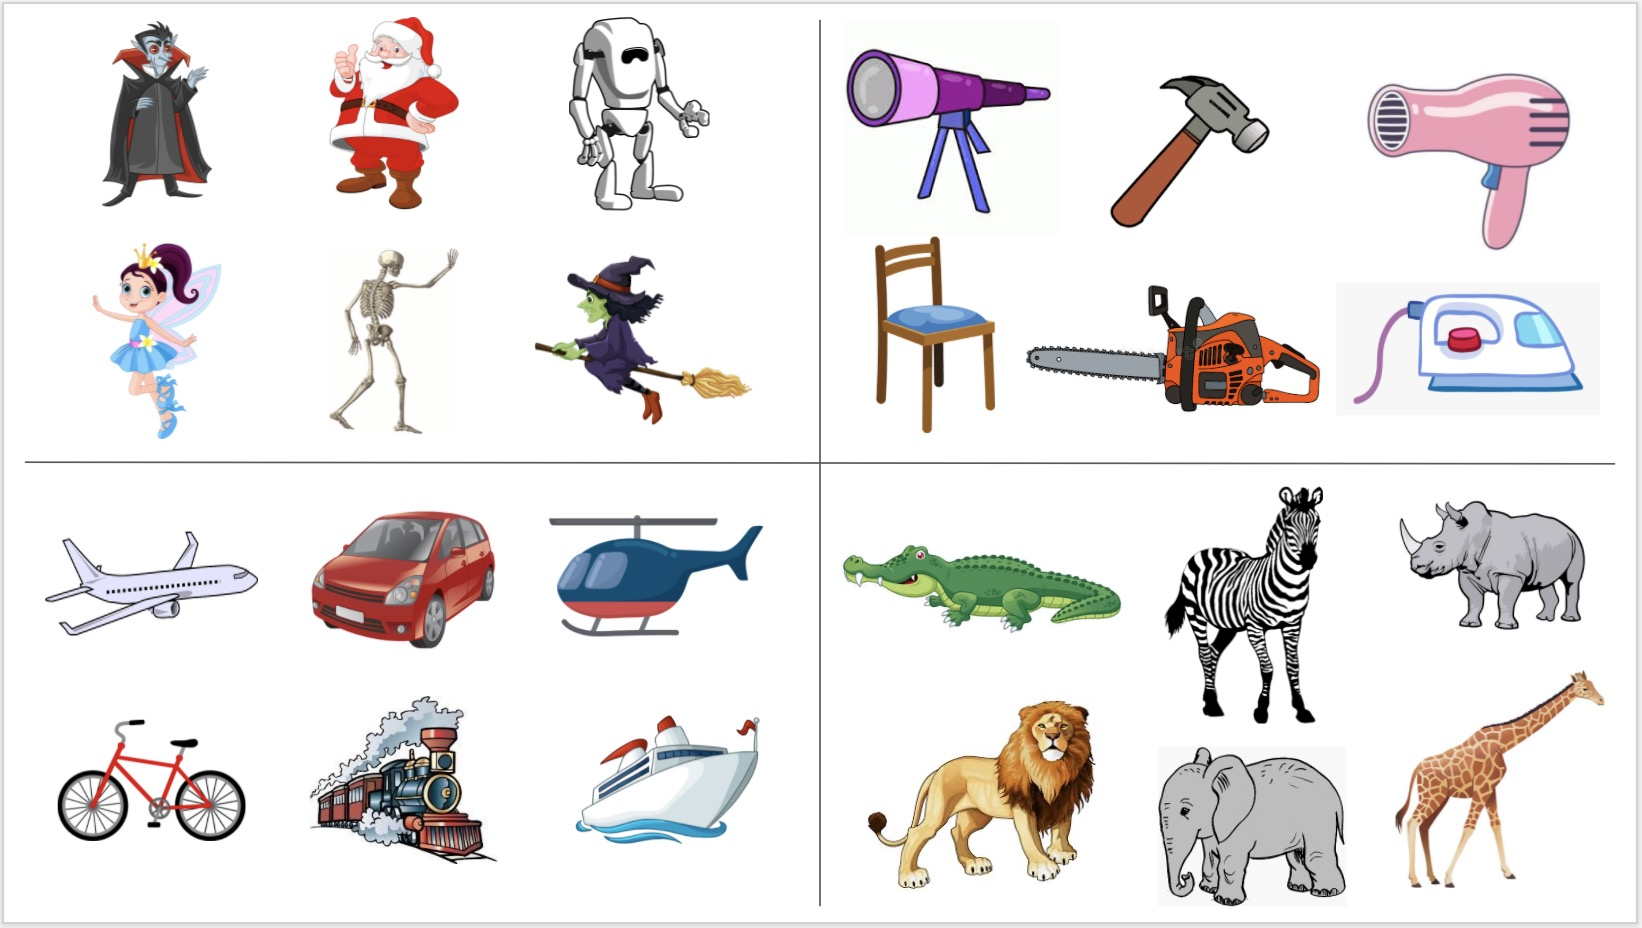
\includegraphics{group-b/E2-example-figure.jpeg}
\caption{\label{fig:E2-example-trial}Example trial from Experiment 2.}
\end{figure}

During the recall phase, participants listened to statements and
responded by pressing the `F' key for false statements and `T' for true
ones. Each statement fell into either an interobject or intraobject
condition. Interobject statements were those that compared two different
items in the grid (e.g.~``The skeleton is to the left of the robot''),
while intraobject statements were those that asked about the orientation
of a single item (e.g.~``The bus is facing right''). There were 48 total
statements, with 24 interobject and 24 intraobject statements split
evenly among the four quadrants. While listening to these statements, in
the free-viewing block, participants saw a blank screen and were allowed
to freely gaze around the screen. During the fixed-viewing block,
participants were asked to fixate a small cross in the center of the
screen throughout the recall phase. In both cases, the mouse was
obscured from the screen. Participants were randomly assigned to see the
fixed-viewing or free-viewing block first. Different images were used in each block.

After completing both encoding-recall blocks, participants were asked to
answer a few survey questions (such as whether they wore glasses or
encountered any distractions).

The primary methodological difference between this replication and
Johansson and Johansson's study was that the original study included two
additional viewing conditions that were omitted from this replication
due to time constraints. In those two conditions, participant were
prompted to look to a specific quadrant (rather than free viewing or
central fixation) which either matched or mismatched the original
location of the to-be-remembered item.

\subsection{Results}\label{results-1}

\subsubsection{Replication}\label{replication}

\textbf{Eye-gaze}. Looks during the retrieval period were categorized as belonging to one of four quadrants based on the x,y coordinates. The critical quadrant was the one in which the to-be-retrieved object had been previously located during encoding. The other three quadrants were semi-randomly labeled ``first'', ``second,'' third'' (e.g., when the critical quadrant was in the top left, the ``first'' quadrant was the top right quadrant, but when the critical quadrant was in the top right, ``first'' corresponded to bottom right, etc.). In both the fixed- and free-viewing condition, participants directed a larger proportion of looks to the critical quadrant (see Figure \ref{fig:E2-gaze-fig-both-conds}). This bias appeared larger in the free-viewing condition, suggesting that the manipulation was (somewhat) effective.

\begin{figure}
\centering
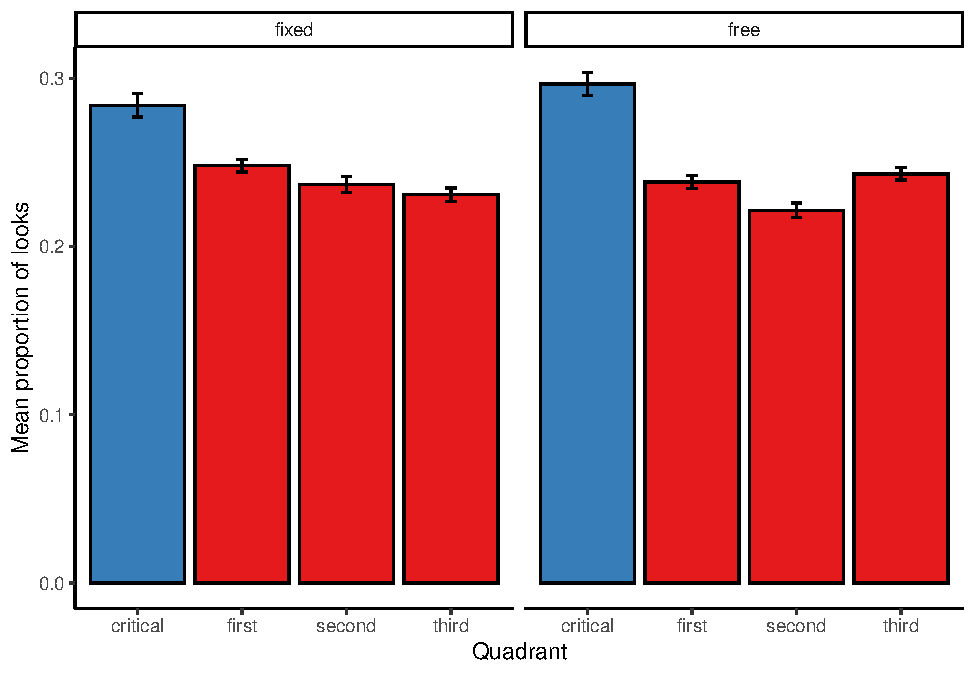
\includegraphics{manuscript_files/figure-latex/E2-gaze-fig-both-conds-1.pdf}
\caption{\label{fig:E2-gaze-fig-both-conds}Proportion of eye-gaze to critical quadrant and other three quadrants during memory retrieval in a) fixed and b) free viewing conditions.}
\end{figure}

The proportions of looks across quadrants in the free-viewing condition were analyzed using a linear mixed-effects model with quadrant as the predictor (critical as the reference level). The model included random intercepts and slopes for participants\footnote{ \texttt{lme4} syntax: \texttt{lmer(proportion\ \textasciitilde{}\ quadrant\ +\ (1+quadrant\textbar{}subject\_id))}. Among other limitations, this approach violates the independence assumptions of the linear model because looks to the four locations are not independent. This analysis was chosen because it is analogous to the ANOVA analysis conducted in the original paper.}. Proportions of looks were significantly higher for the critical quadrant compared to the other three (first: \emph{b} = -0.06, \emph{SE} = 0.01, \emph{p}\textless0.001, second: \emph{b} = -0.08, \emph{SE} = 0.01, \emph{p}\textless0.001, third: \emph{b} = -0.05, \emph{SE} = 0.01, \emph{p}\textless0.001 )

\begin{figure}
\centering
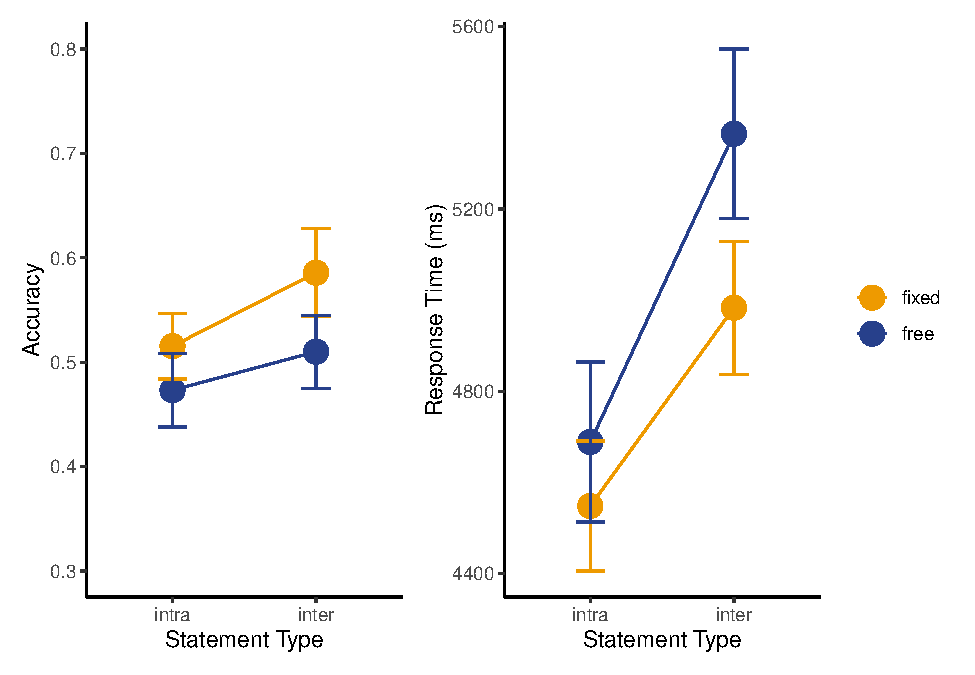
\includegraphics{manuscript_files/figure-latex/E2-rt-acc-fig-1.pdf}
\caption{\label{fig:E2-rt-acc-fig}Accuracy and response times during memory retrieval.}
\end{figure}

\textbf{Response Time and Accuracy}. Participants' response times and accuracies on memory questions are summarized in Figure \ref{fig:E2-rt-acc-fig}.
Both dependent variables were analyzed with linear mixed-effects model with relation type (interobject = -0.5, intraobject=0.5) and viewing\_condition (fixed = -0.5, free=0.5) and their interaction as the predictors.
The model included random intercepts for participants\footnote{ \texttt{lme4} syntax: \texttt{lmer(DV\ \textasciitilde{}\ relation\_type*viewing\_condition\ +\ (1\textbar{}subject\_id))}}.
Accuracy did not differ significantly between interobject and intraobject questions (\emph{b} = -0.05, \emph{SE} = 0.03, \emph{p}=0.05). Participants were less accurate in the free viewing condition than the fixed condition (\emph{b} = -0.06, \emph{SE} = 0.03, \emph{p}=0.03).
Response times were slower for interobject (e.g., ``The train is to the right of the taxi.'') than intraobject (e.g., ``The train is facing right.'') questions (\emph{b} = -555.60, \emph{SE} = 105.24, \emph{p}\textless0.001). Response times were slower in the free viewing condition than the fixed condition (\emph{b} = 260.98, \emph{SE} = 105.24, \emph{p}\textless0.001).
The interaction was not a significant predictor for response times or accuracy.
These behavioral results are inconsistent with the original findings.

One possibility is that in-lab participants were much more compliant with the instruction to keep their gaze on central fixation (though these data are not reported in the original paper). When analyzing results from the subset of participants (N = 25) who were most compliant during the fixed-viewing block (at least 25\% of their looks fell within 20\% of the center of the display), the viewing condition effects and the interactions were not signficant. Given the smaller sample size we do not interpret these results further.

\subsubsection{Calibration}\label{calibration-2}

Participants' calibration quality, measured as the mean percentage of fixations that landed within 200 pixels of the calibration point, varied substantially (between 17.78 and 100 \%).
The quality of a participant's calibration was not significantly correlated with the participant's effect size ( \emph{Pearson's r}= 0.20, \emph{p} = 0.14) as measured by the difference between the proportion of looks to the critical quadrant minues the average proportion of looks to the average of the other three quadrants.

\subsection{Discussion}\label{discussion-1}

As in Johansson and Johansson (2014) and Spivey and Geng (2001), during memory retrieval, learners spontaneously look to blank screen locations where pictures were located
during encoding, suggesting that visuospatial information is integrated into the memory
for objects. However, we did not observe a memory benefit, in terms of speed or accuracy, of spatial reinstatement via gaze position during retrieval of the picture. We can speculate that this may be due to the fact that participants struggled to maintain their gaze fixed in the center in the fixed-viewing condition, such that the difference between the fixed- and free-viewing conditions was minimal. Crucially for the current purposes, the webcam-based eye-tracking measurements were successful in replicating the key eye-tracking results.

\section{Experiment 3}\label{experiment-3}

The third study was a partial replication attempt of
Manns, Stark, and Squire (2000). This experiment used the visual
paired-comparison, which involves presenting a previously-viewed image
and novel image together and measuring the proportion of time spent
looking at each image. The expected pattern of results is that
participants will look more at novel objects. They
Manns et al. (2000) hypothesized that this pattern of
behavior could be used to measure the strength of memories. If a viewer
has a weak memory of the old image, then they may look at the old and
new images roughly the same amount of time. They tested this in two
ways. First, they showed participants a set of images, waited five
minutes, and then paired those images with novel images. They found that
participants spent more time (58.8\% of total time) looking at the novel
images. They then measured memory performance one day later and found
that participants were more likely to recall images that they had spent
less time looking at during the visual paired-comparison task the
previous day.

\subsection{Method}\label{method-2}

The stimuli, experimental code, and data and analysis scripts can be
found on the Open Science Framework at \url{https://osf.io/k63b9/}.
The pre-registration for the study can be
found at \url{https://osf.io/48jsv} . We
inadvertently did not create a formal pre-registration using the OSF
registries tool, but this document contains the same information and is
time stamped prior to the start of data collection.

\subsubsection{Participants}\label{participants-3}

Our pre-registered target was 50 participants. 51 participants completed
the first day of the experiment and 48 completed the second day.
Following Manns et al., we excluded 3 participants due to perfect
performance on the recognition memory test because this prevents
comparison of gaze data for recalled vs.~non-recalled images. Our final
sample size was 45 participants.

\subsubsection{Procedure}\label{procedure-2}

The task began with a 7-point eye-tracker calibration (each point was
presented 3 times in a random order) and validation with 3 points (each
presented once). The point locations were designed to focus calibration
on the center of the screen and the middle of the left and right halves
of the screen (Figure~\ref{fig:E3-calibration-figure}).

\begin{figure}
\centering
\includegraphics{manuscript_files/figure-latex/E3-calibration-figure-1.pdf}
\caption{\label{fig:E3-calibration-figure}Calibration and validation point locations for Experiment 3. Black points were used for calibration. Red crosses were used for checking the accuracy of the calibration.}
\end{figure}

The experiment was administered over the course of two
consecutive days. It consisted of three sections: a presentation phase,
a test phase, and a recognition test. The first two phases occurred on
the first day, while the recognition test occurred on the second day.

During the presentation phase, participants viewed 24 pairs of identical
color photographs depicting common objects. Each pair was presented for
5 seconds and an interval of 5 seconds elapsed before the next pair was
shown. The order of the photographs was randomized and different for
each participant. After completion of the presentation phase,
participants were given a 5-minute break during which they could look
away from the screen.

After the break, they were prompted to complete the eye-tracking
calibration again before beginning the test phase. During this phase,
participants again viewed 24 pairs of photographs with an interstimulus
duration of 5 seconds. In each pair, one photograph was previously seen
during the presentation phase, while the other was new. Which pictures
were old or new was counterbalanced across participants.
For half of the participants in each counterbalancing group, the new and
old photographs were
reversed.

Approximately 24 hours after completing the first session, with a leeway
interval of 12 hours to accommodate busy schedules, participants were
given the recognition test. It consisted of 48 photographs, presented
one at a time. Each was shown on the screen for 1 second, followed by a
1 second interstimulus interval. Half of the photographs had been
viewed twice on the previous day and were deemed the ``targets.'' The
other half depicted an object with the same name as an object in one of
the old photographs, but had not been viewed before, deemed ``foils.''
Each photograph remained on the screen until the participants indicated
whether or not they had seen it before by pressing `y' for yes and `n'
for no. After they pressed one of the two keys, a prompt on the screen
asked them to rate their confidence in their answer from 1 as a ``pure
guess'' to 5 as ``very sure.'' by clicking on the corresponding number on
the screen. No feedback on their responses was given during the test.

The experimental design is visually depicted in Figure~\ref{fig:E3-design-schematic}.

There were two modifications we made to the methods of the original
experiment. As we were only replicating the declarative memory component
of the original experiment, we did not have a ``priming group.''
Therefore, we followed only the procedure for the ``looking group.''
Additionally, for each section of the study, the stimuli were presented
on a single screen instead of two screens due to the constraints of the
online experiment format.

\begin{figure}
\centering
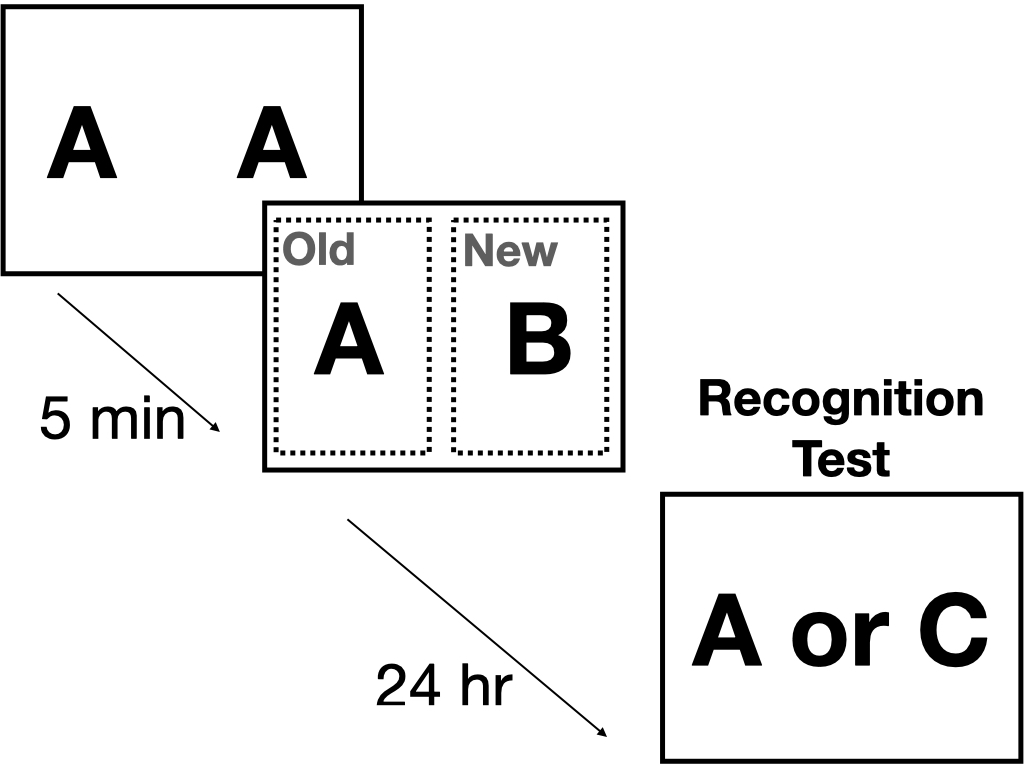
\includegraphics{group-c/E3-example-figure.jpeg}
\caption{\label{fig:E3-design-schematic}Schematic of the design of Experiment 3}
\end{figure}

\subsubsection{Materials}\label{materials}

\textcolor{red}{Images were selected XXX...}

\subsection{Results}\label{results-2}

\paragraph{Day 1}\label{day-1}

During day 1 of the experiment, participants viewed pairs of images, one of which was always familiar and the other unfamiliar. We calculated a looking score for each participant, defined as the proportion of gaze samples in the ROI of the unfamiliar image out of all the gaze samples that were in either ROI. Gaze samples that were not in either ROI were not included in this analysis. A looking score of 0.5 indicates that participants looked equally often at the familiar and unfamiliar images, while a looking score above 0.5 indicates a preference for the unfamiliar object and a looking score below 0.5 indicate a preference for the familiar object.

Of the 1248 trials in the experiment, 78 had no fixations in either ROI, and so the looking score was unknown. We removed these trials from this analysis.

The mean looking score was 0.55 (\emph{SD} = 0.10). This significantly greater than 0.5, \emph{t}(49) = 3.29, \emph{p} = 0.00, indicating that participants did show a preference for looking at the novel objects.

\begin{figure}
\centering
\includegraphics{manuscript_files/figure-latex/plot-cumulative-looking-score-1.pdf}
\caption{\label{fig:plot-cumulative-looking-score}Cumulative looking score over the 5 second exposure during part 2 of day 1. Error bars represent +/- 1 SEM.}
\end{figure}

\paragraph{Day 2}\label{day-2}

In all of these analyses, we excluded the 16 (out of 2304) trials where the response time for the recognition judgment was greater than 10 seconds.

Participants correctly identified whether the image was familiar or unfamiliar 87.09\% (\emph{SD} = 10.49) of the time. After excluding the 3 participants who responded correctly to all images, the average confidence rating for correct responses (M = 3.51; SD = 0.41) was significantly higher than their average confidence ratings for incorrect responses (M = 2.55; SD = 0.75), t(44) = 9.36, p = 0.00 . Among the same subset of participants, response times for correct responses (M = 1,443.49, SD = 413.94) were also significantly faster than for incorrect responses (M = 2,212.65, SD = 1,733.76), t(44) = -3.43 , p = 0.00.

To see whether preferentially looking an the unfamiliar object on day 1 was correlated with confidence and response time for correct responses on day 2, we computed the correlation coefficient between day 1 looking scores and day 2 confidence/RT for each participant. Following the original analysis, we transformed these values using the Fisher p-to-z transformation. Using one-sample t-tests, we found no significant different from 0 for the correlation between looking score and confidence ratings, t(38) = 0.46, p = 0.65 (excluding the subjects who gave the same confidence judgment for all images), nor the the correlation between looking score and RT, t(46) = 0.49, p = 0.63.

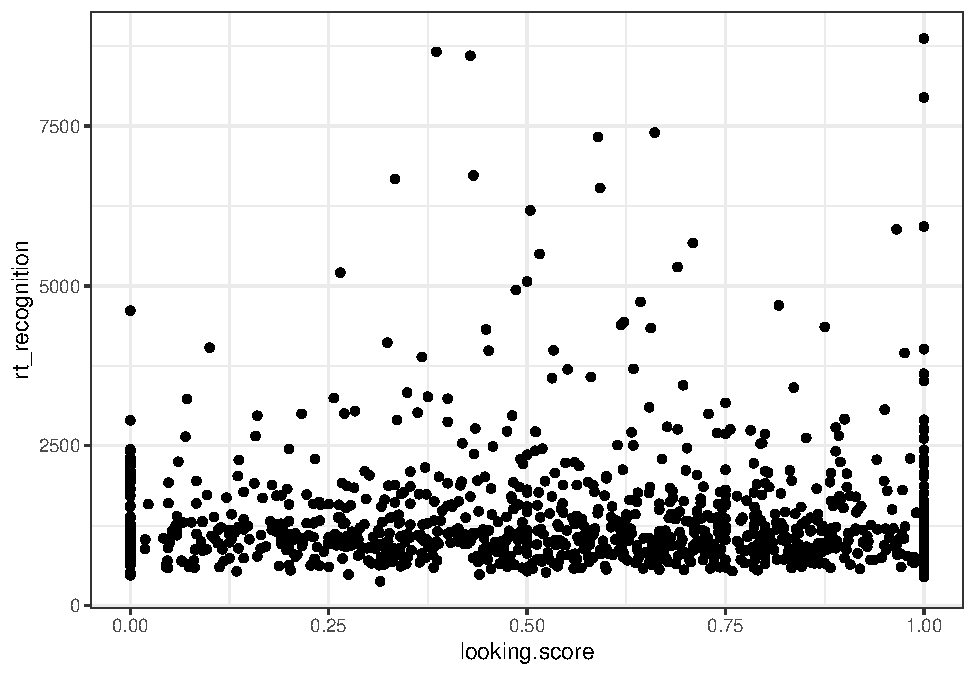
\includegraphics{manuscript_files/figure-latex/Plot Looking Score Correlations-1.pdf}

\subsubsection{Effects of ROIs}\label{effects-of-rois}

In the original experiment, the two objects on day 1 were presented on two separate monitors and gaze was coded by manually coding video recordings. In our replication analysis, we analyzed eye movement data using ROIs defined around the two images. In this section we explore an alternative coding of the eye movement data by coding simply left half vs.~right half of the screen. The coarser coding may be more appropriate for webcam-based eyetracking.

The correlation between looking scores using the ROI method and the halves method is 0.76.

\begin{figure}
\centering
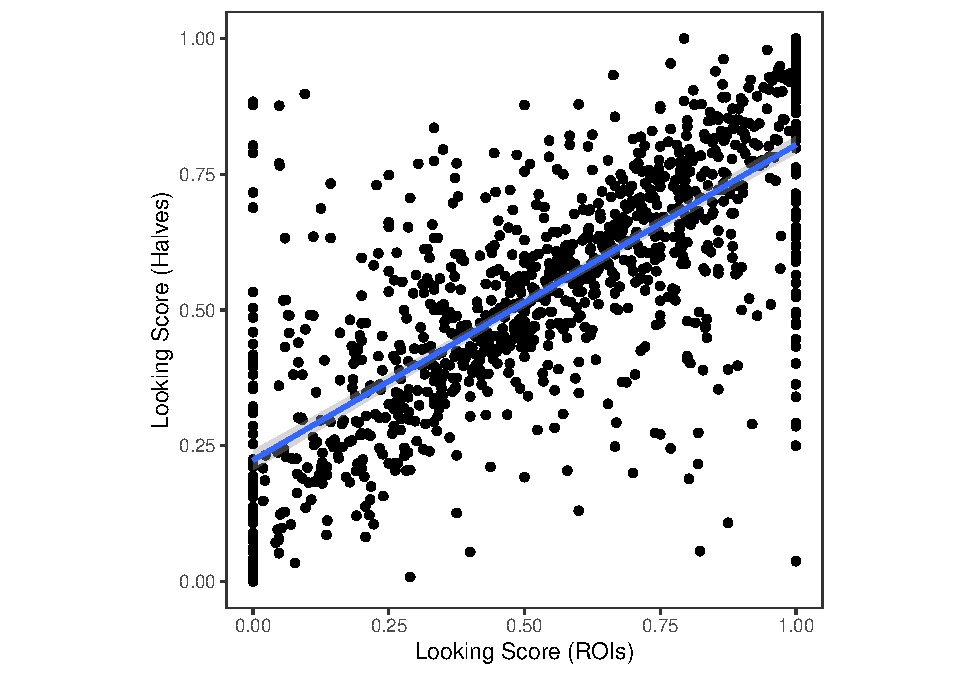
\includegraphics{manuscript_files/figure-latex/E3-roi correlation of looking score-1.pdf}
\caption{(\#fig:E3-roi correlation of looking score)Correlation between looking scores calculated using ROIs and using screen halves.}
\end{figure}

\paragraph{Looking Scores}\label{looking-scores}

When looking scores are coded as left vs.~right half of the screen, we find that participants looked more at the novel object. The mean looking score was 0.54 (\emph{SD} = 0.08). This was significantly greater than 0.5, \emph{t}(50) = 3.51, \emph{p} = 0.00.

\begin{figure}
\centering
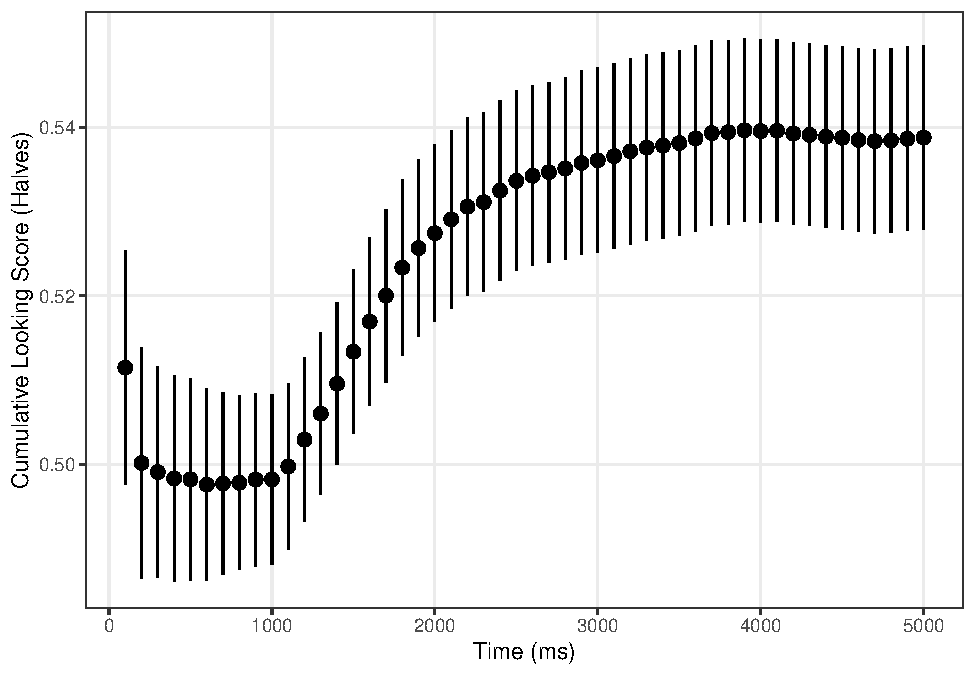
\includegraphics{manuscript_files/figure-latex/E3-roi Plot of cumulative looking score-1.pdf}
\caption{(\#fig:E3-roi Plot of cumulative looking score)Cumulative looking score over the 5 second exposure during part 2 of day 1. Error bars represent +/- 1 SEM.}
\end{figure}

\paragraph{Correlations with Day 2 Performance}\label{correlations-with-day-2-performance}

Performance on day 2 remained uncorrelated with day 1 looking scores after switching the coding of gaze. We found no significant different from 0 for the correlation between looking score and confidence ratings, t(39) = 0.74, p = 0.47 (excluding the subjects who gave the same confidence judgment for all images), nor the the correlation between looking score and RT, t(47) = 0.28, p = 0.78.

\subsubsection{Calibration}\label{calibration-3}

\paragraph{Calibration Accuracy}\label{calibration-accuracy}

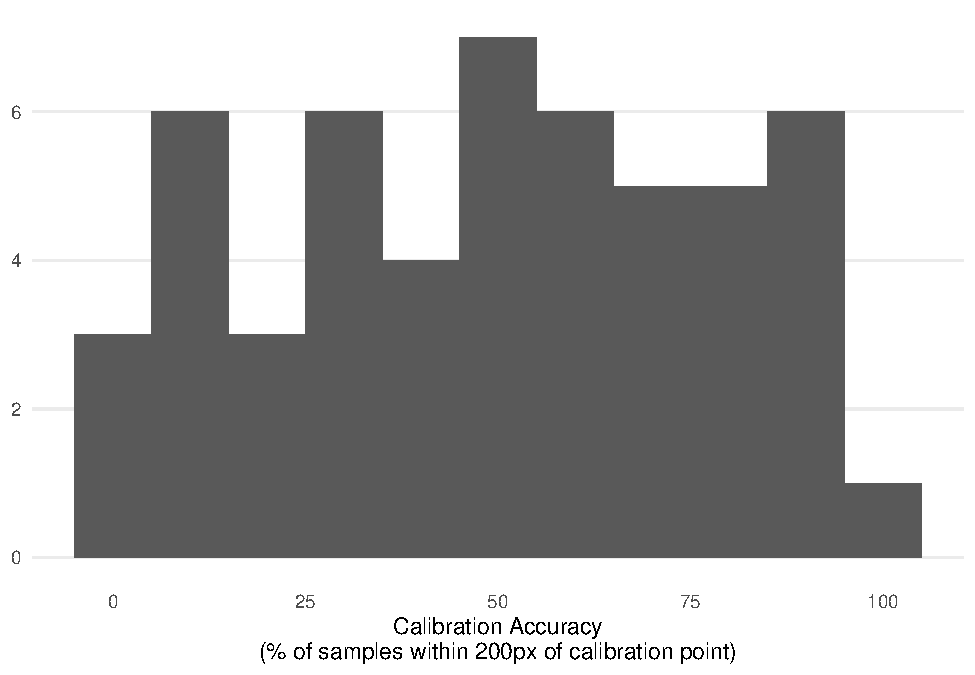
\includegraphics{manuscript_files/figure-latex/E3-cal Plot Calibration Accuracy-1.pdf}

\paragraph{Correlation with Effects}\label{correlation-with-effects}

To see if calibration success is correlated with the eye tracking effects, we calculated a calibration score for each participant. The calibration score was the average proportion of samples within 200 pixels of the validation points during the final validation phase before the eye tracking is performed.

Calibration scores were not correlated with looking scores, regardless of which method was used to calculate looking scores.

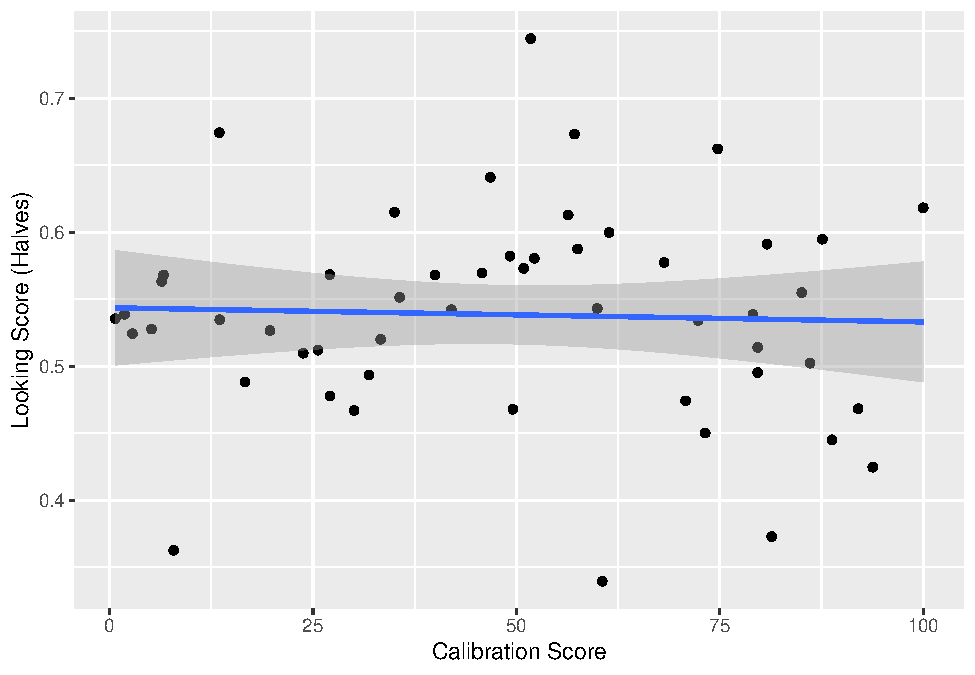
\includegraphics{manuscript_files/figure-latex/E3-cal Plot looking score (halves) by calibration-1.pdf}

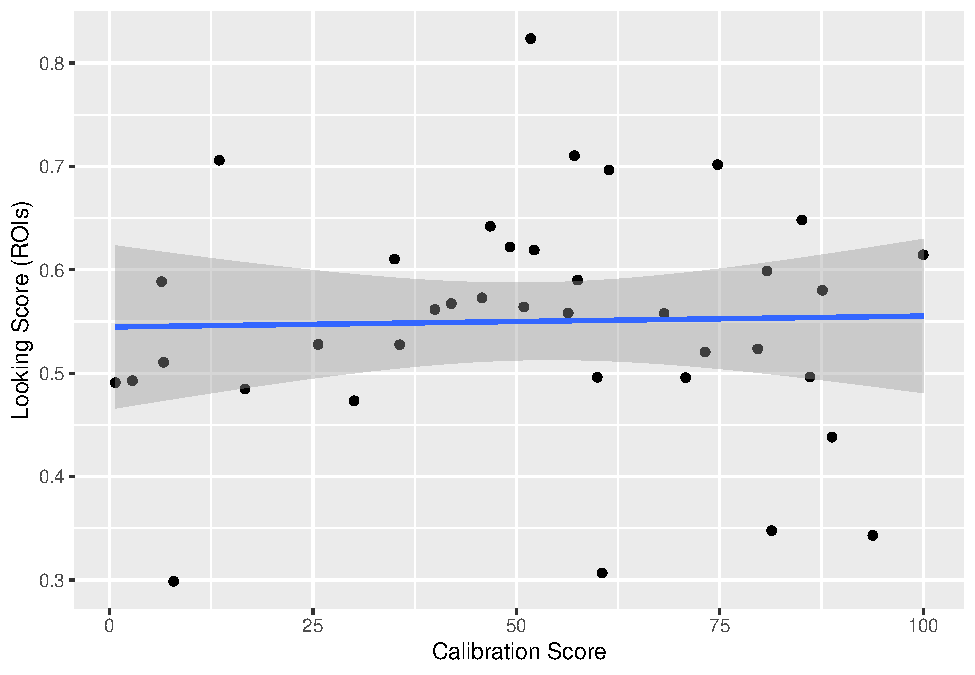
\includegraphics{manuscript_files/figure-latex/E3-cal Plot looking score (roi) by calibration-1.pdf}

We then looked at the correlation of calibration scores with the correlation between day 2 memory performance and day 1 looking scores for both kinds of behavioral and looking measures. None of the four relationships showed a significant correlation.

\includegraphics{manuscript_files/figure-latex/E3-cal Plot correlations with calibration score-1.pdf}

\subsection{Discussion}\label{discussion-2}

As in Manns et al. (2000), participants looked more at novel images than previously seen images. This effect was consistent for ROIs based on the images and for the coarser ROIs based on two halves of the display. A day later, participants were also able to discriminate the images they had seen from foil images they had not seen during the previous session. However, there was no evidence that memory performance on day 2 was related to looking time on day 1. Calibration quality did not appear to impact this relationship.

\section{Experiment 4}\label{experiment-4}

The fourth study was a replication attempt of Experiment 1 in
Ryskin, Qi, Duff, and Brown-Schmidt (2017), which was closely modeled on
Snedeker and Trueswell (2004). These studies used the
visual world paradigm to show that listeners use knowledge of the
co-occurrence statistics of verbs and syntactic structures to resolve
ambiguity. For example, in a sentence like ``Feel the frog with the
feather,'' the phrase ``with the feather'' could be describing the frog, or
it could be describing the instrument that should be used to do the
``feeling.'' When both options (a frog holding a feather and a feather by
itself) are available in the visual display, listeners rely on the
verb's ``bias'' (statistical co-occurrence either in norming or corpora)
to rapidly choose an action while the sentence is unfolding. .

\subsection{Method}\label{method-3}

The stimuli, experimental code, and data and original analysis scripts can be
found on the Open Science Framework at the following link,
\url{https://osf.io/x3c49/}. The pre-registration
for the study can be found at \url{https://osf.io/3v4pg}.

\subsubsection{Participants}\label{participants-4}

57 participants were paid \$2.50 for their participation. A sample size of 60 was initially chosen (but not reached in time) because we wanted to replicate the experiment with greater statistical power. Note that the original study had a sample size of 24.

\subsubsection{Procedure}\label{procedure-3}

After the eye-tracking calibration and validation (Figure~\ref{fig:E4-calibration-figure}), participants went through an audio
test so they could adjust the audio on their computer to a comfortable
level. Before beginning the experiment, they were given instructions
that four objects would appear, an audio prompt would play, and they
should do their best to use their mouse to act out the instructions.
They then went through three practice trials which were followed by 54
critical trials and 24 filler trials presented in a random order.

\begin{figure}
\centering
\includegraphics{manuscript_files/figure-latex/E4-calibration-figure-1.pdf}
\caption{\label{fig:E4-calibration-figure}Calibration and validation point locations for Experiment 4. Black points were used for calibration. Red crosses were used for checking the accuracy of the calibration.(In this experiment all the same locations were used for both calibration and validation.)}
\end{figure}

During a trial, four pictures were displayed (target animal, target
instrument, distractor animal, distractor instrument), one in each
corner of the screen, and participants heard an audio prompt that
contained instructions about the action they needed to act out (e.g.,
``Rub the butterfly with the crayon''; see Figure~\ref{fig:E4-example-trial})\footnote{In the original study, the pictures appeared one by one on the
  screen and their names were played as they appeared. We removed this
  introductory portion of the trial to save time}. Using their
cursor, participants could act out the instructions by clicking on
objects and moving them or motioning over the objects\footnote{As opposed to the original study we recorded mouse movement
  instead of clicking behavior since not all of the audio prompts
  required clicking. For example, the sentence ``locate the camel with
  the straw'' may not involve any clicking but rather only mousing over
  the camel.}. After the
action was completed, the participants were instructed to press the
space bar which led to a screen that said ``Click Here'' in the middle in
order to remove bias in the eye and mouse movements from the previous
trial. The experiment only allowed the participants to move on to the
next trial once the audio was completely done playing and the mouse had
been moved over at least one object.

\begin{figure}
\centering
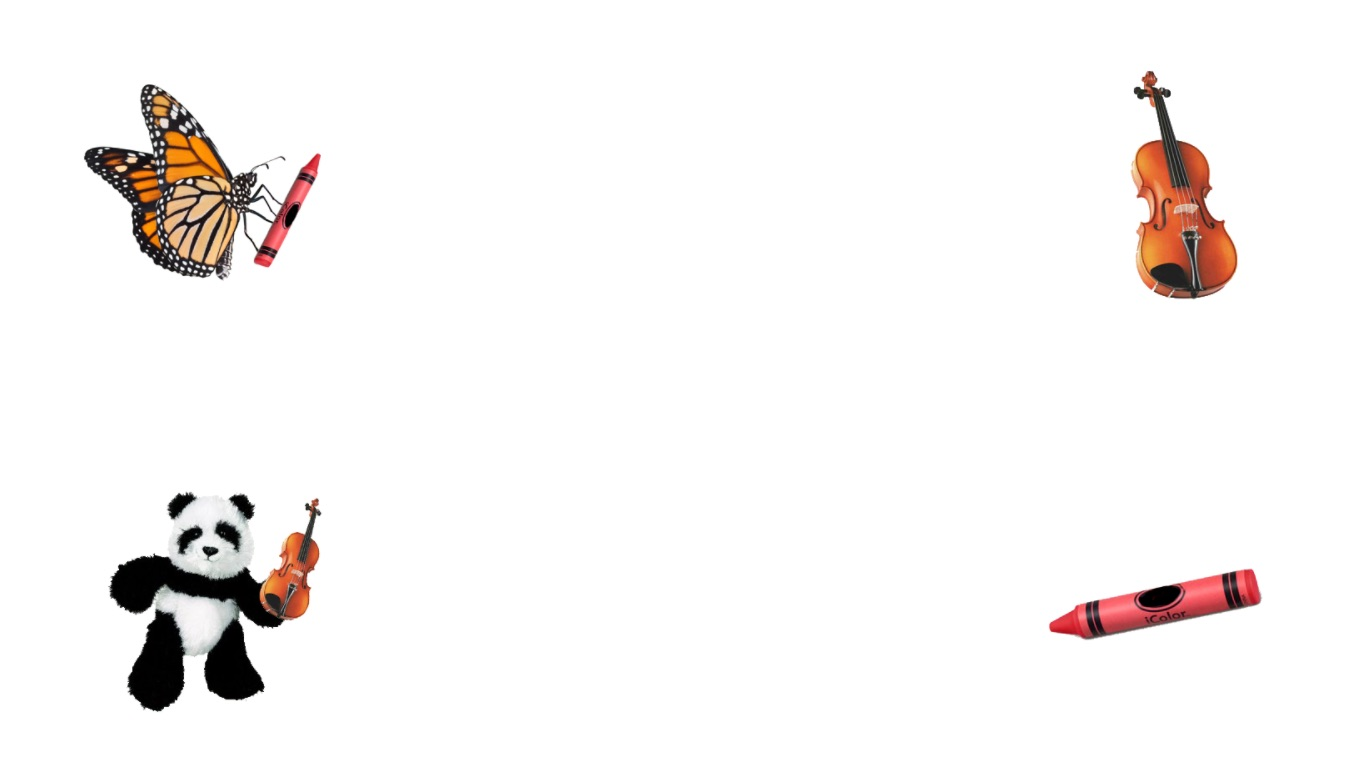
\includegraphics{group-d/E4-example-figure.jpeg}
\caption{\label{fig:E4-example-trial}An example of a critical trial from Experiment 4 for the sentence ``Rub the butterfly with the crayon.'' The butterfly is the target animal, the panda is the distractor animal, the crayon is the target instrument, and the violin is the distractor instrument.}
\end{figure}

\subsubsection{Materials}\label{materials-1}

The images and audios presented to the participants were the same
stimuli used in the original study (available here ). The critical
trials were divided into modifier-biased, instrument-biased, and
equibiased conditions, and the filler trials did not contain ambiguous
instructions. Two lists of critical trials were made with different verb
and instrument combinations (e.g., ``rub'' could be paired with ``panda''
and ``crayon'' in one list and ``panda'' and ``violin'' in the second list).
Within each list, the same verb was presented twice but each time with a
different target instrument and animal. The lists were randomly assigned
to the participants to make sure the effects were not caused by the
properties of the animal or instrument images used. The list of verbs
used can be found in Appendix A of the original study.

\subsection{Results}\label{results-3}

\subsubsection{Replication}\label{replication-1}

The location of initial mouse movements was used to assess whether the final interpretation of ambiguous sentences was biased by the verb. Figure \ref{fig:E4-mouse-moves-fig} suggests that listeners were more likely to move their mouse first over the target instrument when the verb was equi-biased than when the verb was modifier-biased and even more so when the verb was instrument-biased. The opposite graded pattern can be observed for mouse movements over the target animal.

\begin{figure}
\centering
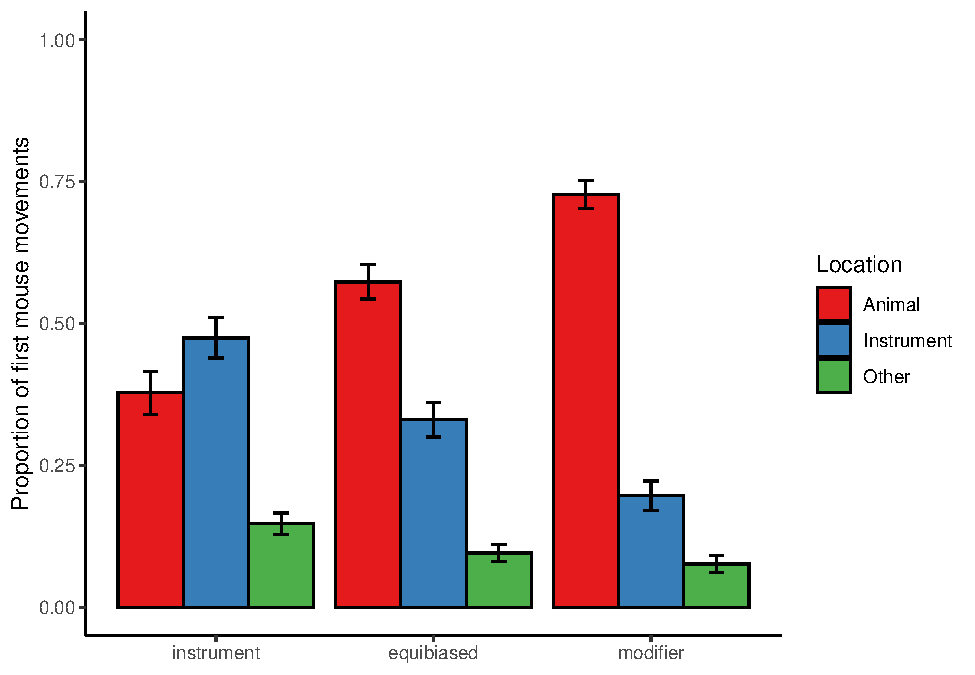
\includegraphics{manuscript_files/figure-latex/E4-mouse-moves-fig-1.pdf}
\caption{\label{fig:E4-mouse-moves-fig}Proportion of first mouse movements by location and verb bias.}
\end{figure}

A mixed-effects logistic regression model was used to predict whether the first movement was on the target instrument with the verb bias condition as an orthogonally contrast-coded (instrument vs.~equi \& modifier: inst = -2/3, equi = 1/3, mod = 1/3; equi vs.~modifier: inst = 0, equi = -1/2, mod = 1/2 ) fixed effect. Participants and items were entered as varying intercepts with by-participant varying slopes for verb bias condition\footnote{\texttt{lme4} syntax: \texttt{glmer(is.mouse.over.instrument\ \textasciitilde{}\ verb\_bias\ +\ (1\ +\ verb\_bias\ \textbar{}\ participant)\ +\ (1\ \textbar{}\ item),\ family="binomial",\ data=d)}}. Participants were more likely to first move their mouse over target instruments in the instrument-biased condition relative to the equi-biased and modifier-biased condition (\emph{b} = -1.50, \emph{SE} = 0.25, \emph{p} \textless{} 0.01). Further, participants were more likely to first move their mouse over target instruments in the equi-biased condition relative to the modifier-biased condition (\emph{b} = -1.10, \emph{SE} = 0.29, \emph{p} \textless{} 0.01)

Gaze fixations were time-locked to the auditory stimulus on a trial by trial basis and categorized as being directed towards one of the four items in the display if the x, y coordinates fell within a rectangle containing the image. Figure \ref{fig:E4-gaze-timecourse-fig} suggests that the participants made more fixations to the target animal when the verb was modifier-biased compared to when the the verb was equi-biased and they looked at the target animal least when the verb was instrument-biased. The pattern was reversed for looks to the target instrument.

\begin{figure}
\centering
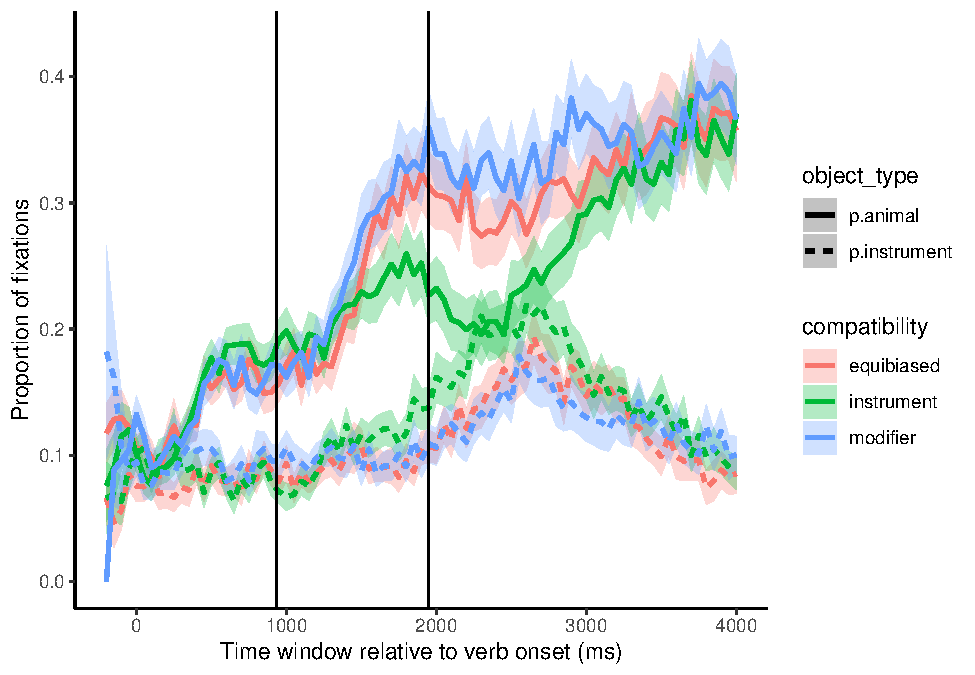
\includegraphics{manuscript_files/figure-latex/E4-gaze-timecourse-fig-1.pdf}
\caption{\label{fig:E4-gaze-timecourse-fig}Timecourse of eye-gaze to target animal and target instrument by verb bias condition. Vertical lines indicate average onsets of animal and instrument offset by 200ms.}
\end{figure}

In order to assess how verb bias impacted sentence disambiguation as the sentence unfolded, the proportion of fixations was computed in three time windows: the verb-to-animal window (from verb onset + 200 ms to animal onset + 200 ms), the animal-to-instrument window (from animal onset + 200 ms to instrument onset + 200 ms), and the post-instrument window (from instrument onset + 200 ms to instrument onset + 1500ms + 200 ms). Mixed-effects linear regression models were used to predict the proportions of fixations to the target animal within each time window with the verb bias condition as an orthogonally contrast-coded (instrument vs.~equi \& modifier: inst = -2/3, equi = 1/3, mod = 1/3; equi vs.~modifier: inst = 0, equi = -1/2, mod = 1/2 ) fixed effect. Participants and items were entered as varying intercepts\footnote{\texttt{lme4} syntax: \texttt{lmer(prop.fix.target.animal\ \textasciitilde{}\ verb\_bias\ +\ (1\ +\ verb\_bias\ \textbar{}\ participant)\ +\ (1\ \textbar{}\ item),\ data=d)}. A model with by-participant varying slopes for verb bias condition was first attempted but did not converge.}. In the \emph{verb-to-noun} window, participants did not look more at the target animal in any of the verb bias conditions (Instrument vs.~Equi and Modifier: \emph{b} = -0.01, \emph{SE} = 0.02, \emph{p} = 0.59; Equi vs.~Modifier: \emph{b} = 0, \emph{SE} = 0.02, \emph{p} = 1 ). In the \emph{noun-to-instrument} window, participants looked more at the target animal in the modifier-biased condition and equi-biased conditions relative to the instrument-biased condition ( \emph{b} = 0.03, \emph{SE} = 0.01, \emph{p} \textless{} 0.01) and in the modifier biased relative to the equi-biased condition ( \emph{b} = 0.02, \emph{SE} = 0.01, \emph{p} \textless{} 0.05). In the \emph{post-instrument} window, participants looked more at the target animal in the modifier-biased condition and the equi-biased conditions relative to the instrument-biased condition ( \emph{b} = 0.08, \emph{SE} = 0.02, \emph{p} \textless{} 0.01) but not significantly so in the modifier biased condition relative to the equi-biased condition ( \emph{b} = 0.03, \emph{SE} = 0.02, \emph{p} = 0.15).

\subsubsection{Comparison to in-lab data}\label{comparison-to-in-lab-data}

The web version of the study qualitatively replicates the action and eye-tracking results of the original dataset (Ryskin et al., 2017).
The mouse click results from both studies are summarized in Figure \ref{fig:E4-mouse-moves-fig-web-and-orig}.
The quantitative patterns of clicks were similar to those observed in the original dataset, though for Instrument-biased verbs, clicks were closer to evenly split between the animal and the instrument relative to the in-lab study where they were very clearly biased toward the instrument.

\begin{figure}
\centering
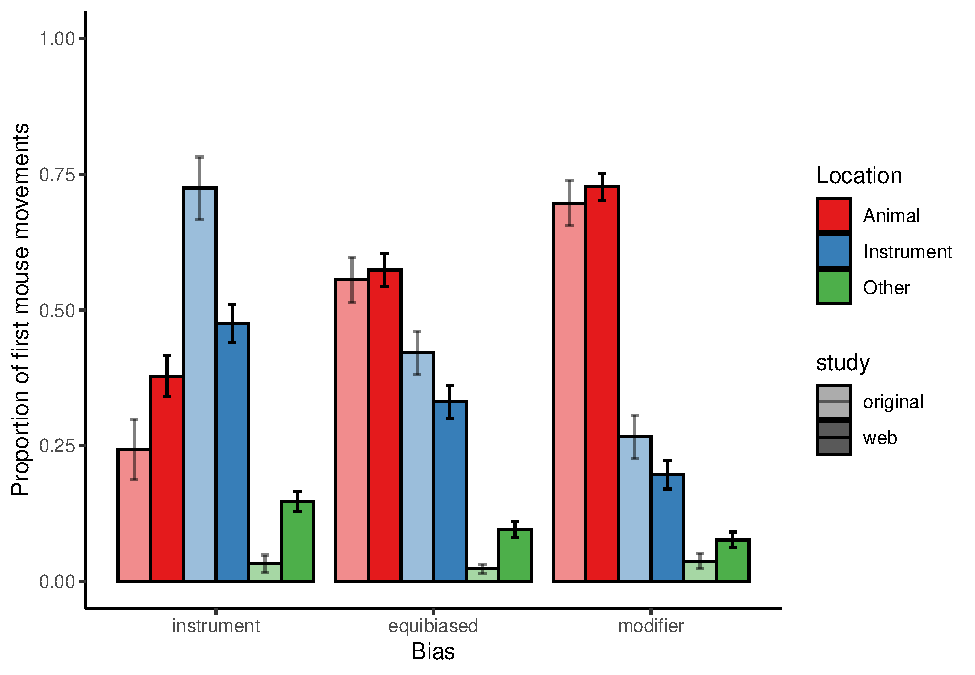
\includegraphics{manuscript_files/figure-latex/E4-mouse-moves-fig-web-and-orig-1.pdf}
\caption{\label{fig:E4-mouse-moves-fig-web-and-orig}Proportion of first mouse movements by location and verb bias in the original dataset (Ryskin et al., 2017) and the current data collected online.}
\end{figure}

The eye-tracking results from both studies are summarized in Figure \ref{fig:E4-proportion-fix-by-window-both}.
For simplicity, and to reflect the dependent variable used in analyses, we average the proportion of fixations to the target animal within each time window.
Though the qualitative patterns are replicated, proportions of fixations to the target animal were much lower in the web version of the study.
This may reflect the fact that participants in the web study are less attentive and/or the quality of the webgazer eye-tracking system is lower, relative to the Eyelink 1000 which was used for the original study.

\begin{figure}
\centering
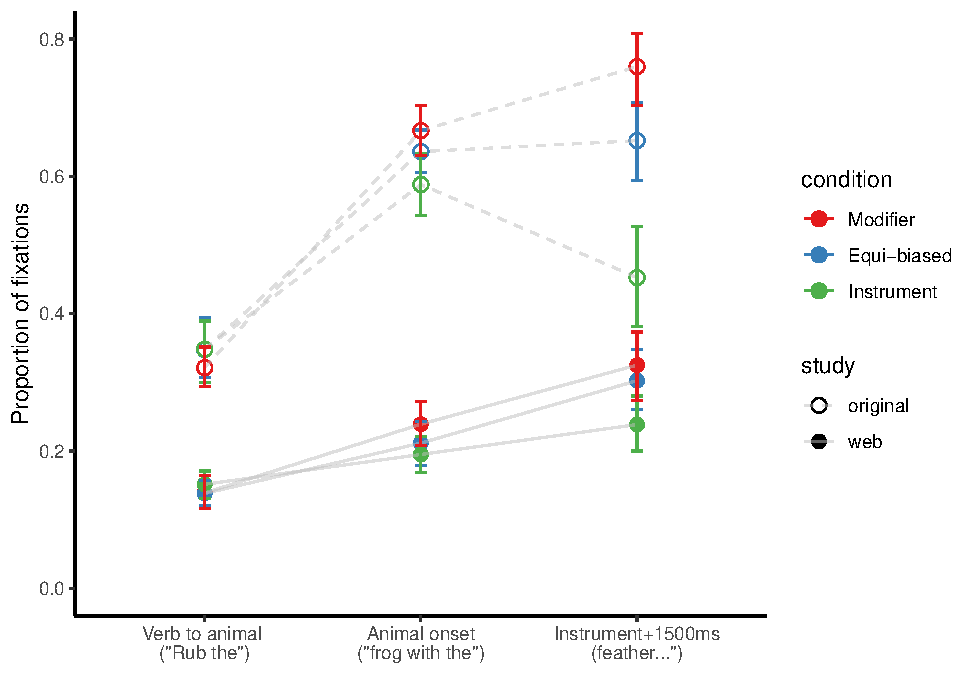
\includegraphics{manuscript_files/figure-latex/E4-proportion-fix-by-window-both-1.pdf}
\caption{\label{fig:E4-proportion-fix-by-window-both}Proportion of target fixations by verb bias in the original dataset (Ryskin et al., 2017) and the current data collected online. Error bars reflect bootstrapped 95\% CIs over subject means}
\end{figure}

\subsubsection{Calibration}\label{calibration-4}

Participants' calibration quality, measured as the mean percentage of fixations that landed within 200 pixels of the calibration point, varied substantially (between 2.22 and 97.36 \%).
The quality of a participant's calibration significantly correlated with the participant's effect size ( \emph{Pearson's r}= 0.29, \emph{p} \textless{} 0.05).
The difference in target animal fixation proportions between modifier and instrument conditions was higher for participants with better calibration

Replicating the linear mixed-effects analysis (in the post-instrument onset time window only) on a subset of 35 participants with calibration quality \textgreater50\% suggests that the effect of verb bias condition was larger in this subset than in the full dataset. Participants looked more at the target animal in the modifier-biased condition and the equi-biased conditions relative to the instrument-biased condition ( \emph{b} = 0.10, \emph{SE} = 0.02, \emph{p} \textless{} 0.001) but not significantly so in the modifier biased condition relative to the equi-biased condition ( \emph{b} = 0.02, \emph{SE} = 0.02, \emph{p} = 0.29).

Replicating the linear mixed-effects analysis (in the post-instrument onset time window only) on a subset of 19 participants with calibration quality \textgreater75\% suggests that the effect of verb bias condition was larger in this subset than in the full dataset.
Participants looked more at the target animal in the modifier-biased condition and the equi-biased conditions relative to the instrument-biased condition ( \emph{b} = 0.11, \emph{SE} = 0.03, \emph{p} \textless{} 0.001) but not significantly so in the modifier biased condition relative to the equi-biased condition ( \emph{b} = 0.05, \emph{SE} = 0.03, \emph{p} = 0.13).

\subsubsection{Effects of ROIs}\label{effects-of-rois-1}

Eye-tracking on the web differs critically from in-lab eye-tracking in that the size of the display differs across participants. Thus the size of the ROIs differs across participants. The current version of the web experiment used a bounding box around each image to determine the ROI.
This approach is flexible and accomodates variability in image size, but may exclude looks that are directed at the image but fall outside of the image (due to participant or eye-tracker noise) as show in Figure \ref{fig:E4-example-subj-looks-ROI}a. Alternatively, The display can be split into 4 quadrants which jointly cover the entire screen (see Figure \ref{fig:E4-example-subj-looks-ROI}b).

\begin{figure}
\centering
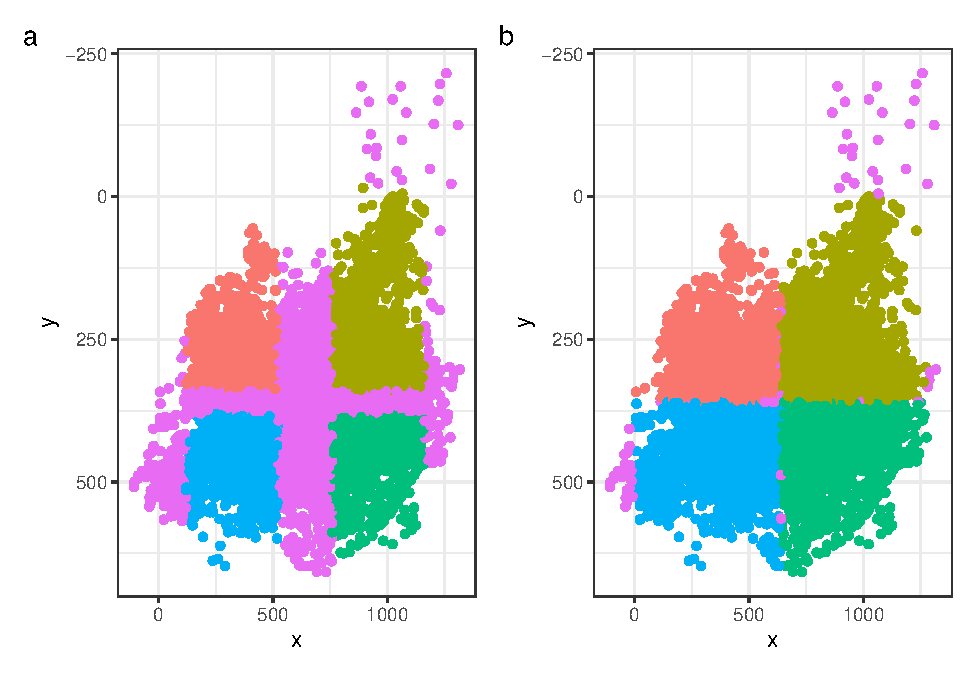
\includegraphics{manuscript_files/figure-latex/E4-example-subj-looks-ROI-1.pdf}
\caption{\label{fig:E4-example-subj-looks-ROI}Example participant's gaze coordinates categorized into ROIs based on a) image bounding boxes and b) screen quadrants. Magenta points indicate looks that were not categorized into an ROI}
\end{figure}

\begin{figure}
\centering
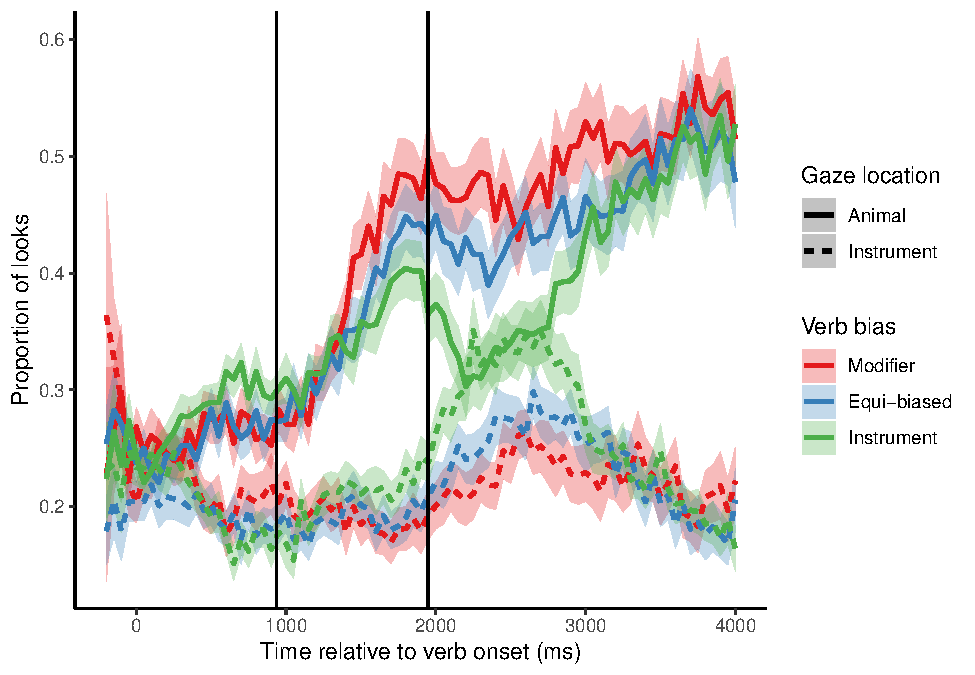
\includegraphics{manuscript_files/figure-latex/E4-gaze-timecourse-fig-quadrants-1.pdf}
\caption{\label{fig:E4-gaze-timecourse-fig-quadrants}Timecourse of eye-gaze to target animal and target instrument by verb bias condition with gaze categorized based on which quadrant of the screen the coordinates fall in (as opposed to a bounding box around the image). Vertical lines indicate average onsets of animal and instrument offset by 200ms.}
\end{figure}

Categorizing gaze location based on which of the four quadrants of the screen the coordinates fell in, increases the overall proportions of fixations (see Figure \ref{fig:E4-gaze-timecourse-fig-quadrants}). In the \emph{post-instrument} window, participants looked more at the target animal in the modifier-biased condition and the equi-biased conditions relative to the instrument-biased condition ( \emph{b} = 0.08, \emph{SE} = 0.02, \emph{p} \textless{} 0.01) and marginally so in the modifier biased condition relative to the equi-biased condition ( \emph{b} = 0.04, \emph{SE} = 0.02, \emph{p} = 0.05). Effect size estimates appeared somewhat larger and noise was somewhat reduced when using the quadrant categorization relative to the bounding box-based ROIs.

\subsection{Discussion}\label{discussion-3}

As in Ryskin et al. (2017) and Snedeker and Trueswell (2004), listeners' gaze patterns during sentences with globally ambiguous syntactic interpretations differed depending on the bias of the verb (i.e., modifier, instrument or equi). For modifier-biased verbs, participants looked more quickly at the target animal and less at the potential instrument than for instrument-biased verbs (and equi-biased verbs elicited a gaze pattern between these extremes). This pattern was stronger for those who achieved higher calibration accuracy and when quadrant-based ROIs were used compared to image-based ROIs.

\section{Experiment 5}\label{experiment-5}

The fifth study was a replication attempt of Shimojo et al. (2003),
which found that human gaze is actively involved in preference
formation. Separate sets of participants were shown pairs of human faces
and asked either to choose which one they found more attractive or which
they felt was rounder. Prior to making their explicit selection,
participants were increasingly likely to be fixating the face they
ultimately chose, though this effect was significantly weaker for
roundness discrimination.

Note that Shimojo and colleagues compare five conditions, of which we
replicate only the two that figure most prominently in their
conclusions: the ``face-attractiveness-difficult task'' and the
``face-roundness task''.

\subsection{Method}\label{method-4}

All stimuli, experiment scripts, data, and analysis scripts are
available on the Open Science Framework at \url{https://osf.io/eubsc/}.
The study pre-registration is available at
\url{https://osf.io/tv57s}.

\subsubsection{Participants}\label{participants-5}

50 participants for the main task were recruited on Prolific and were
paid \$10/hour. 8 subjects, 4 from the attractiveness task group and 4 from
the roundness task group, were excluded for incorrect validations.
After this
data exclusion, we ended up with 21 participants each for the
attractiveness task and the roundness task. The original sample size in
Shimojo et al.~(2003) was 10 participants total.

\subsubsection{Procedure and Design}\label{procedure-and-design}

At the beginning of the experimental task, participants completed a
9-point eye-tracker calibration (each point appeared 3 times in random
order) and 3-point validation. The validation point appeared once at
center, middle left, and middle right locations in random order (see Figure~\ref{fig:E5-calibration-figure}).

\begin{figure}
\centering
\includegraphics{manuscript_files/figure-latex/E5-calibration-figure-1.pdf}
\caption{\label{fig:E5-calibration-figure}Calibration and validation point locations for Experiment 5. Black points were used for calibration. Red crosses were used for checking the accuracy of the calibration.}
\end{figure}

During each trial of the main task, two faces were displayed on the two
halves of the screen, one on the left and one on the right (as in Figure~\ref{fig:E5-example-trial}). Participants were randomly assigned to one of two tasks:
attractiveness or shape judgment. In the attractiveness task,
participants were asked to chose the more attractice face in the pair
and in the shape judgment task participants were asked to pick the face
that appeared rounder. They pressed the ``a'' key on their keyboard to
select the face on the left and the ``d'' key to select the face on the
right. A fixation cross appeared in the center of the screen between
each set of faces. Participants were asked to look at this fixation
cross in order to reset their gaze in between trials. The order of
the 19 face pairs was random for each participant.

\begin{figure}
\centering
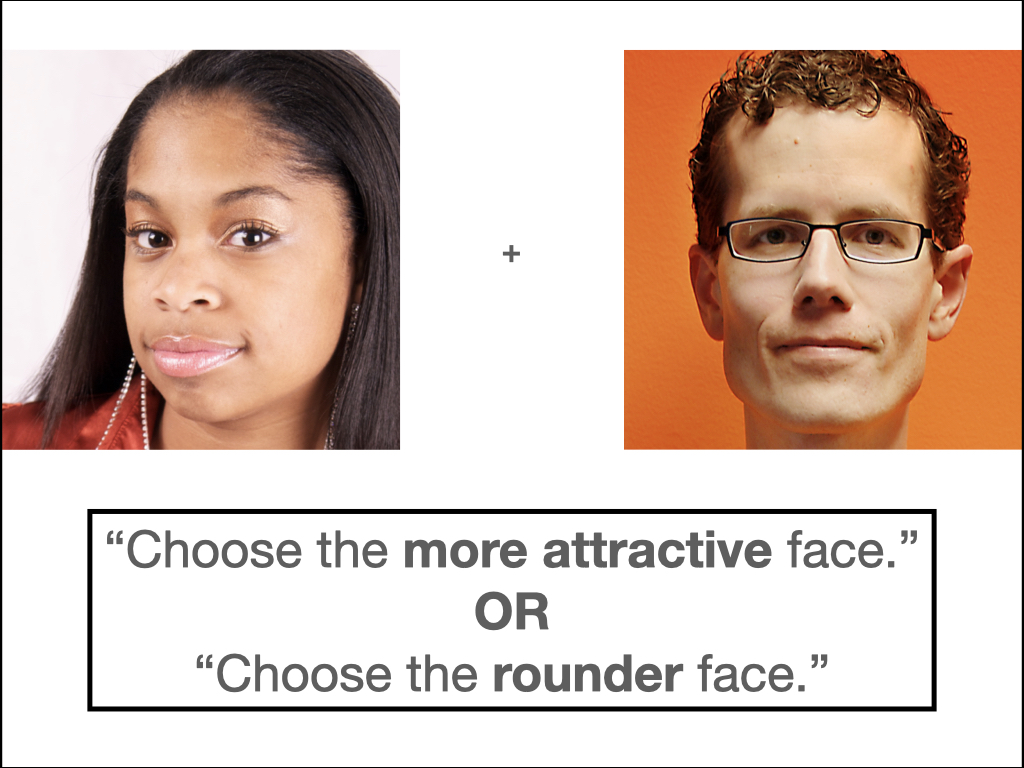
\includegraphics{group-e/E5-example-figure.jpeg}
\caption{\label{fig:E5-example-trial}An example of a critical trial from Experiment 5. (Text did not appear on each screen.)}
\end{figure}

\subsubsection{Materials and Norming}\label{materials-and-norming}

The faces in our replication were selected from a set of 1,000 faces
within the Flickr-Faces-HQ Dataset. (The face images used in Shimojo et
al.~were from the Ekman face database and the AR face database.) These
images were chosen because the person in each image was looking at the
camera with a fairly neutral facial expression and appeared to be over
the age of 18. 27 participants were recruited on Prolific to participate
in stimulus norming (for attractiveness). They each viewed all 172 faces and were asked to rate
them on a scale from 1 (less attractive) to 7 (more attractive) using a
slider. Faces were presented one at a time and in a random order for
each participant. Data from 3 participants were excluded because
their mode response made up more than 50\% of their total responses, for a total of 24 participants
in the norming.

Following Shimojo et al., 19 face pairs were selected by
identifying two faces that 1) had a difference in mean attractiveness ratings
that was 0.25 points or lower and 2) matched in gender, race, and age
group (young adult, adult, or older adult).

\subsubsection{Data analysis}\label{data-analysis}

In the original study, a video-based eye tracker was used. The eye
movements of participants were recorded with a digital camera
downsampled to 33.3 Hz, with eye position was then determined
automatically with MediaAnalyzer software. In our study, subjects
supplied their own cameras, so hardware sampling rate varied. However,
data was collected at 20 Hz.\textcolor{red}{[TODO - CONFIRM]}

\subsection{Results}\label{results-4}

Due to large variation in response time latency, Shimojo and colleagues analyzed eye gaze for the 1.67 seconds prior to the response. This duration was one standard deviation of the mean response time, ensuring that all timepoints analyzed have data from at least 67\% of trials. In our dataset, one standard deviation amounts to 1.85 seconds. We then binned eyegaze data into 50 ms bins rather than the 30 ms bins used by Shimojo and colleagues, reflecting the different sampling rates.



\begin{figure}
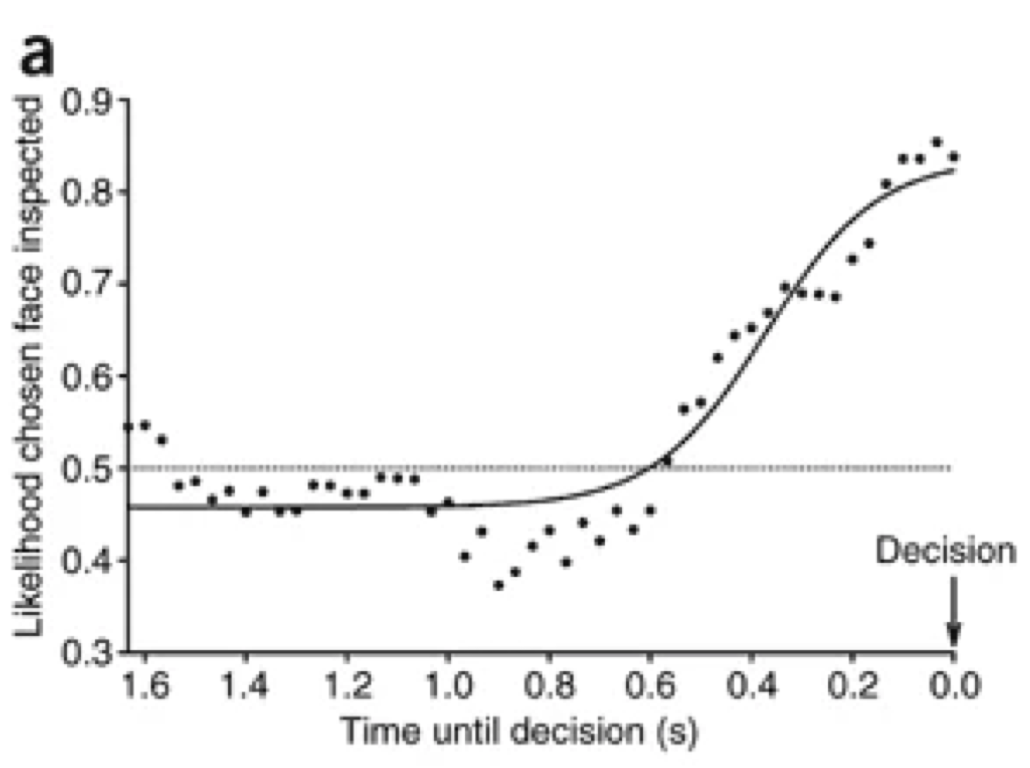
\includegraphics[width=0.45\linewidth]{figGroupEOrigA} 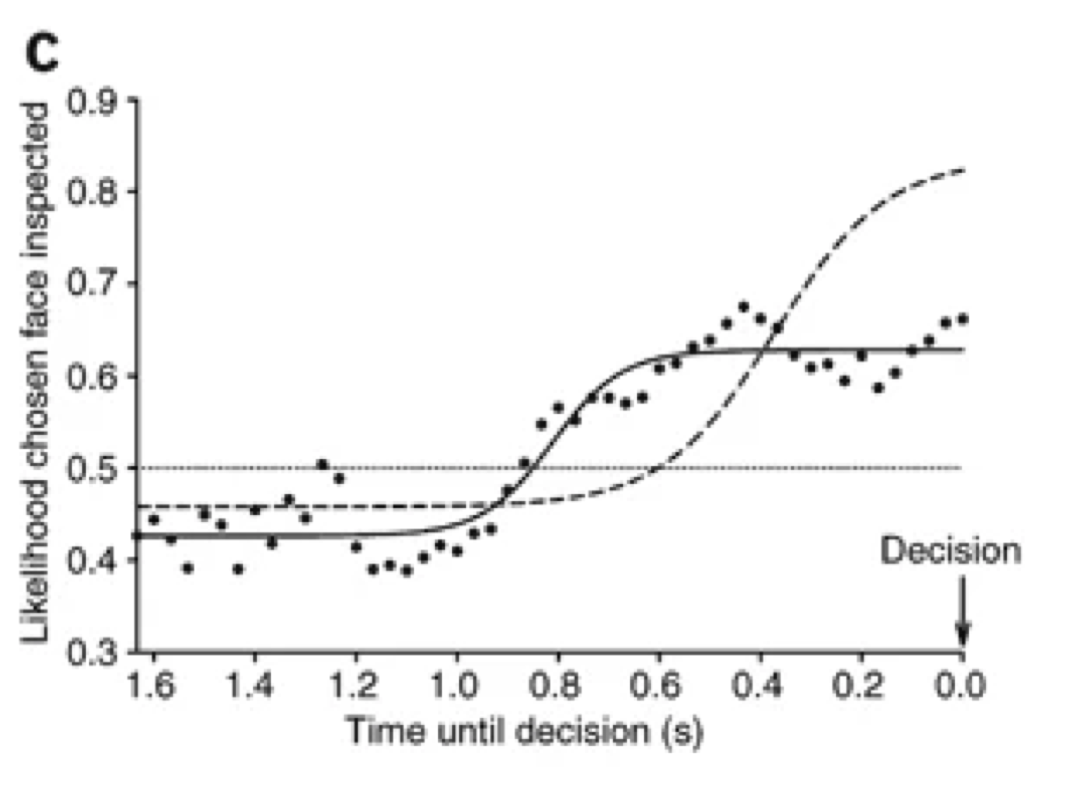
\includegraphics[width=0.45\linewidth]{figGroupEOrigB} \includegraphics[width=0.45\linewidth]{manuscript_files/figure-latex/groupEMain-3} \includegraphics[width=0.45\linewidth]{manuscript_files/figure-latex/groupEMain-4} \caption{Primary results from Exp. 5. \emph{Top} shows the original results from Shimojo and colleagues (Figures reprinted with permission{[}TODO{]}). The attractiveness judgment along with the best-fitting sigmoid is shown in the \emph{top left}. Results for the roundness judgment are show in the \emph{top right}, with the best-fitting sigmoid for the attractiveness judgment depicted in a dashed line for comparison (\emph{top right}). (\emph{Bottom}) shows the analogous results from the replication, with the attractiveness judgments on the \emph{bottom left} and the roundness judgments on the \emph{bottom right}. Again, the best-fitting sigmoid for the attractiveness judgments are plotted with a dashed line alongside the roundness results, for purposes of comparison.}\label{fig:groupEMain}
\end{figure}

Following Shimojo and colleagues, data for each condition were fit using a four-parameter sigmoid (Fig. \ref{fig:groupEMain}). These fit less well than in the original paper for both the attractiveness judgment (R\textsuperscript{2} = 0.84 vs.~0.91) and the roundness judgment (R\textsuperscript{2} = 0.54 vs.~0.91).

From these curves, Shimojo and colleagues focus on two qualitative findings. First, they note a higher asymptote for the attractiveness discrimination task relative to roundness discrimination. Qualitatively, this appears to replicate. However, their statistical analysis -- a Kolmogorov-Smirnov test for distance between two distributions -- is not significant (D = 0.19, p = 0.53), though it should be noted that this is a very indirect statistical test of the hypothesis and probably not very sensitive.

The second qualitative finding they note is that the curve for the roundness judgment ``saturates'' (asymptotes) earlier than the curve for the attractiveness judgment. They do not present any statistical analyses, but it is clear qualitatively that the result does not replicate.

\subsubsection{Calibration}\label{calibration-5}

As in the previous experiments, calibration score was defined as the average proportion of samples within 200 pixels of the validation point during the final validation phase before the eye tracking is performed. The distribution across participants is shown in Fig. \ref{fig:E5cal}.


\begin{figure}
\includegraphics[width=0.45\linewidth]{manuscript_files/figure-latex/E5cal-1} \caption{Histogram of calibration success in Exp. 5. Where participants required more than one calibration (N=8), only the final calibration was considered.}\label{fig:E5cal}
\end{figure}

To determine whether calibration accuracy influenced our key effects, we calculated the percentage of samples during the task in which the participant was fixating the face they ultimately chose. There was a significant correlation for both the attractiveness judgments (r = 0.47 {[}0.04, 0.75{]}, p = 0.03) and the roundness judgments (r = 0.60 {[}0.23, 0.82{]}, p = 0). Inspection of Fig. \ref{fig:E5calcorr} reveals that this correlation is due to a handful of particpiants with calibration values below 50\%.



\begin{figure}
\includegraphics[width=0.8\linewidth]{manuscript_files/figure-latex/E5calcorr-1} \caption{Correlation between calibration accuracy (x-axis) and percentage of samples fixating target (y-axis) in Exp. 5.}\label{fig:E5calcorr}
\end{figure}

Thus, we re-analyzed the data, removing the participants whose calibration accuracy was not greater than 50\%. This slightly improved the fits of the sigmoids (Attractiveness: R\textsuperscript{2} = 0.79; Roundness: R\textsuperscript{2} = 0.60). However, the difference between sigmoids remained non-significant using the Kolmogorov-Smirnov test (D = 0.22, p = 0.36). Descriptively, the results do not look substantially different (Fig. \ref{fig:groupEMainrev}).



\begin{figure}
\includegraphics[width=0.45\linewidth]{manuscript_files/figure-latex/groupEMainrev-1} \includegraphics[width=0.45\linewidth]{manuscript_files/figure-latex/groupEMainrev-2} \caption{Revised results for Exp. 5 after removing low-calibration accuracy participants. \emph{Left}: Eyegaze during attractiveness judgments, along with the best-fitting sigmoid. \emph{Right}: Eyegze during roundness judgments, along with best-fitting sigmoid (best-fitting sigmoid for attractiveness is re-plotted with a dashed line for comparison).}\label{fig:groupEMainrev}
\end{figure}

\subsubsection{Effects of ROIs}\label{effects-of-rois-2}

In the original experiment, eye gazes that did not directly fixate one or other of the faces were excluded. In this section we explore an alternative coding of the eye movement data by coding simply left half vs.~right half of the screen. The coarser coding may be more appropriate for webcam-based eyetracking.

Only a small percentage of samples (7.00\%) involved looks to anything other than one of the two faces. Thus, not surprisingly, the correlation between percentage of time spent fixating the to-be-chosen face using the ROI method and the halves method was near ceiling (r = 0.97 {[}0.97, 0.98{]}, p = 0). Since the choice of method had almost no effect on whether participants were coded as fixating one face or the other, we did not further investigate the effect of method choice on the analytic results.

\subsection{Discussion}\label{discussion-4}

Qualitatively, the results are similar to those of Shimojo et al., such that participants look more at the option that they ultimately choose. This gaze bias appears to be stronger for decisions about face attractiveness than shape, though this is not supported by the statistical analysis approach used in the original paper. The gaze patterns remained consistent for participants with better calibration accuracy.

\section{General Discussion}\label{general-discussion}

We conducted five attempted replication studies using different experimental paradigms from across the cognitive sciences. All were successfully implemented in \texttt{jsPsych} using the \texttt{webgazer} plugin, but replication success was mixed. Experiment 1 had the smallest ROIs due to the use of an integrated visual scene with five to six ROIs of varying size per scene, as opposed to ROIs corresponding to display halves or quadrants. Both attempts to replicate Altmann and Kamide (1999) were unsuccessful, despite the success of previous in-lab replications using infrared eye-tracking (e.g. James et al., 2023). A previous conceptual replication of this paradigm using webcam-based eye-tracking (Prystauka et al., 2023) was successful but used a four-quadrant visual world paradigm, rather than the ``naturalistic'' scenes used in the original study and in the current replication attempts. It is worth noting that removing variability related to participant environments (by conducting the webcam-tracking study in the lab) did not appear to improve the sensitivity of the paradigm. The primary limitation is likely to be the size of the ROIs.

Experiment 2 used the four quadrants of the participant's screen as ROIs. As in Johansson and Johansson (2014) and Spivey and Geng (2001), participants spontaneously looked to blank ROIs which previously contained to-be-remembered pictures. These results appeared to be robust to calibration quality. An additional manipulation, instructing participants to keep gaze fixed on a central point, was not successful. One possibility is that participants are less motivated to follow such instructions when an experimenter is not present in the same room with them. It may be possible to improve performance by emphasizing that this is an important aspect of the experiment or by providing additional training/practice in keeping the eyes still on one particular point.

Experiment 3 used two large ROIs (halves of the display in one analysis) and successfully replicated the novelty preference in terms of gaze duration shown in Manns et al. (2000). However, the subtler relationship between gaze duration and recognition memory on Day 2 was not replicated, despite the fact that participants were able to discriminate pictures they had seen from those they hadn't seen during that delayed test. Calibration quality did not appear to impact this relationship. More work is needed to understand whether delay manipulations can be practically combined with webcam eye-tracking.

Experiment 4 used the four quadrants of the participant's screen as ROIs. As in Ryskin et al. (2017), listeners used knowledge of the co-occurrence statistics of verbs and syntactic structures to resolve ambiguous linguistic input (``Rub the frog with the mitten''). Across multiple time windows, participants looked more at potential instruments (mitten), when the verb (rub) was one that was more likely to be followed by a prepositional phrase describing an instrument with which to perform the action , as opposed to describing the recipient of the action (frog). Despite the qualitative replication of past findings, the overall rates of looks to various objects were much lower than in an in-lab study using infrared eye-tracking. This reduction may be related to measurement quality: effect sizes were greater for participants with higher calibration accuracy. Using the full quadrants as ROIs, rather than bounding boxes around the four images, also appeared to improve the measurement of the effect. Crucially, there was no evidence of a delay in the onset of effects relative to in-lab work, indicating that the modifications to \texttt{webgazer} that are made within the \texttt{jsPsych} plug-in successfully address the issues noted by Dijkgraaf et al. (2017) and suggesting that this methodology can be fruitfully used to investigate research questions related to the timecourse of processing.

Experiment 5, similar to Experiment 3, used two large ROIs (or halves of the display). As in Shimojo et al. (2003) and in the recent webcam-based replication by Yang and Krajbich (2021), we saw that participants looked more at the face or shape that they ultimately chose during a judgment task. This gaze bias appears to be stronger for decisions about face attractiveness than shape, though this effect was not statistically significant.

In sum, the \texttt{webgazer} plug-in for \texttt{jsPsych} can be fruitfully used to conduct a variety of cognitive science experiments on the web, provided the limitations of the methodology are carefully considered. Studies with ROIs that take up half or a quarter of the participant's display, which encompasses a large number of common paradigms, are very likely to be successful, even when testing questions related to the timecourse of processing. However, the smaller the ROIs, the more important the calibration becomes. For instance, studies with four ROIs may want to exclude data from participants with less than 75\% validation accuracy, whereas studies using two halves of the display as ROIs may not need to be so conservative. Studies with smaller ROIs (see Experiment 1) may not be appropriate for webcam eye-tracking in its current form.

\newpage

\section{References}\label{references}

\begingroup
\setlength{\parindent}{-0.5in}
\setlength{\leftskip}{0.5in}

\phantomsection\label{refs}
\begin{CSLReferences}{1}{0}
\bibitem[\citeproctext]{ref-altmannIncrementalInterpretationVerbs1999}
Altmann, G. T. M., \& Kamide, Y. (1999). Incremental interpretation at verbs: Restricting the domain of subsequent reference. \emph{Cognition}, \emph{73}(3), 247--264. \url{https://doi.org/10.1016/S0010-0277(99)00059-1}

\bibitem[\citeproctext]{ref-anwyl2020gorilla}
Anwyl-Irvine, A. L., Massonnié, J., Flitton, A., Kirkham, N., \& Evershed, J. K. (2020). Gorilla in our midst: An online behavioral experiment builder. \emph{Behavior Research Methods}, \emph{52}, 388--407.

\bibitem[\citeproctext]{ref-R-papaja}
Aust, F., \& Barth, M. (2020). \emph{{papaja}: {Create} {APA} manuscripts with {R Markdown}}. Retrieved from \url{https://github.com/crsh/papaja}

\bibitem[\citeproctext]{ref-banki2022comparing}
Bánki, A., Eccher, M. de, Falschlehner, L., Hoehl, S., \& Markova, G. (2022). Comparing online webcam-and laboratory-based eye-tracking for the assessment of infants' audio-visual synchrony perception. \emph{Frontiers in Psychology}, \emph{12}, 733933.

\bibitem[\citeproctext]{ref-R-tinylabels}
Barth, M. (2022). \emph{{tinylabels}: Lightweight variable labels}. Retrieved from \url{https://cran.r-project.org/package=tinylabels}

\bibitem[\citeproctext]{ref-R-lme4}
Bates, D., Mächler, M., Bolker, B., \& Walker, S. (2015). Fitting linear mixed-effects models using {lme4}. \emph{Journal of Statistical Software}, \emph{67}(1), 1--48. \url{https://doi.org/10.18637/jss.v067.i01}

\bibitem[\citeproctext]{ref-R-Matrix}
Bates, D., \& Maechler, M. (2021). \emph{Matrix: Sparse and dense matrix classes and methods}. Retrieved from \url{https://CRAN.R-project.org/package=Matrix}

\bibitem[\citeproctext]{ref-R-broom.mixed}
Bolker, B., \& Robinson, D. (2020). \emph{Broom.mixed: Tidying methods for mixed models}. Retrieved from \url{https://CRAN.R-project.org/package=broom.mixed}

\bibitem[\citeproctext]{ref-R-shiny}
Chang, W., Cheng, J., Allaire, J., Sievert, C., Schloerke, B., Xie, Y., \ldots{} Borges, B. (2021). \emph{Shiny: Web application framework for r}. Retrieved from \url{https://CRAN.R-project.org/package=shiny}

\bibitem[\citeproctext]{ref-deleeuwJsPsychJavaScriptLibrary2015}
de Leeuw, J. R. (2015). {jsPsych}: {A JavaScript} library for creating behavioral experiments in a {Web} browser. \emph{Behavior Research Methods}, \emph{47}(1), 1--12. \url{https://doi.org/10.3758/s13428-014-0458-y}

\bibitem[\citeproctext]{ref-degen2021seeing}
Degen, J., Kursat, L., \& Leigh, D. D. (2021). Seeing is believing: Testing an explicit linking assumption for visual world eye-tracking in psycholinguistics. \emph{Proceedings of the Annual Meeting of the Cognitive Science Society}, \emph{43}.

\bibitem[\citeproctext]{ref-dijkgraaf2017predicting}
Dijkgraaf, A., Hartsuiker, R. J., \& Duyck, W. (2017). Predicting upcoming information in native-language and non-native-language auditory word recognition. \emph{Bilingualism: Language and Cognition}, \emph{20}(5), 917--930.

\bibitem[\citeproctext]{ref-hayhoe2005eye}
Hayhoe, M., \& Ballard, D. (2005). Eye movements in natural behavior. \emph{Trends in Cognitive Sciences}, \emph{9}(4), 188--194.

\bibitem[\citeproctext]{ref-henderson2017meaning}
Henderson, J. M., \& Hayes, T. R. (2017). Meaning-based guidance of attention in scenes as revealed by meaning maps. \emph{Nature Human Behaviour}, \emph{1}(10), 743--747.

\bibitem[\citeproctext]{ref-henninger2021lab}
Henninger, F., Shevchenko, Y., Mertens, U. K., Kieslich, P. J., \& Hilbig, B. E. (2021). Lab. Js: A free, open, online study builder. \emph{Behavior Research Methods}, 1--18.

\bibitem[\citeproctext]{ref-henrich2010weirdest}
Henrich, J., Heine, S. J., \& Norenzayan, A. (2010). The weirdest people in the world? \emph{Behavioral and Brain Sciences}, \emph{33}(2-3), 61--83.

\bibitem[\citeproctext]{ref-james2023language}
James, A. N., Minnihan, C. J., \& Watson, D. G. (2023). Language experience predicts eye movements during online auditory comprehension. \emph{Journal of Cognition}, \emph{6}(1).

\bibitem[\citeproctext]{ref-johanssonLookHereEye2014}
Johansson, R., \& Johansson, M. (2014). Look {Here}, {Eye Movements Play} a {Functional Role} in {Memory Retrieval}. \emph{Psychological Science}, \emph{25}(1), 236--242. \url{https://doi.org/10.1177/0956797613498260}

\bibitem[\citeproctext]{ref-krajbich2010visual}
Krajbich, I., Armel, C., \& Rangel, A. (2010). Visual fixations and the computation and comparison of value in simple choice. \emph{Nature Neuroscience}, \emph{13}(10), 1292--1298.

\bibitem[\citeproctext]{ref-kukona2014lexical}
Kukona, A., Cho, P. W., Magnuson, J. S., \& Tabor, W. (2014). Lexical interference effects in sentence processing: Evidence from the visual world paradigm and self-organizing models. \emph{Journal of Experimental Psychology: Learning, Memory, and Cognition}, \emph{40}(2), 326.

\bibitem[\citeproctext]{ref-R-lmerTest}
Kuznetsova, A., Brockhoff, P. B., \& Christensen, R. H. B. (2017). {lmerTest} package: Tests in linear mixed effects models. \emph{Journal of Statistical Software}, \emph{82}(13), 1--26. \url{https://doi.org/10.18637/jss.v082.i13}

\bibitem[\citeproctext]{ref-mannsVisualPairedcomparisonTask2000}
Manns, J. R., Stark, C. E. L., \& Squire, L. R. (2000). The visual paired-comparison task as a measure of declarative memory. \emph{Proceedings of the National Academy of Sciences}, \emph{97}(22), 12375--12379. \url{https://doi.org/10.1073/pnas.220398097}

\bibitem[\citeproctext]{ref-R-jsonlite}
Ooms, J. (2014). The jsonlite package: A practical and consistent mapping between JSON data and r objects. \emph{arXiv:1403.2805 {[}Stat.CO{]}}. Retrieved from \url{https://arxiv.org/abs/1403.2805}

\bibitem[\citeproctext]{ref-papoutsaki2016webgazer}
Papoutsaki, A., Sangkloy, P., Laskey, J., Daskalova, N., Huang, J., \& Hays, J. (2016). {WebGazer}: {Scalable} webcam eye tracking using user interactions. \emph{Proceedings of the 25th International Joint Conference on Artificial Intelligence ({IJCAI})}, 3839--3845. {AAAI}.

\bibitem[\citeproctext]{ref-prystauka2023online}
Prystauka, Y., Altmann, G. T., \& Rothman, J. (2023). Online eye tracking and real-time sentence processing: On opportunities and efficacy for capturing psycholinguistic effects of different magnitudes and diversity. \emph{Behavior Research Methods}, 1--19.

\bibitem[\citeproctext]{ref-R-base}
R Core Team. (2021). \emph{R: A language and environment for statistical computing}. Vienna, Austria: R Foundation for Statistical Computing. Retrieved from \url{https://www.R-project.org/}

\bibitem[\citeproctext]{ref-rayner1998eye}
Rayner, K. (1998). Eye movements in reading and information processing: 20 years of research. \emph{Psychological Bulletin}, \emph{124}(3), 372.

\bibitem[\citeproctext]{ref-richardsonEyeTrackingResearch2004}
Richardson, D. C., \& Spivey, M. J. (2004). Eye tracking: {Research} areas and applications. In G. Wnek \& G. Bowlin (Eds.), \emph{Encyclopedia of biomaterials and biomedical engineering} (Vol. 572). New York: Marcel Dekker.

\bibitem[\citeproctext]{ref-ryskinVerbBiasesAre2017}
Ryskin, R., Qi, Z., Duff, M. C., \& Brown-Schmidt, S. (2017). Verb biases are shaped through lifelong learning. \emph{Journal of Experimental Psychology: Learning, Memory, and Cognition}, \emph{43}(5), 781--794. \url{https://doi.org/10.1037/xlm0000341}

\bibitem[\citeproctext]{ref-ryskin2023real}
Ryskin, R., Salinas, M., Piantadosi, S., \& Gibson, E. (2023). Real-time inference in communication across cultures: Evidence from a nonindustrialized society. \emph{Journal of Experimental Psychology: General}, \emph{152}(5), 1245.

\bibitem[\citeproctext]{ref-semmelmann2018online}
Semmelmann, K., \& Weigelt, S. (2018). Online webcam-based eye tracking in cognitive science: A first look. \emph{Behavior Research Methods}, \emph{50}, 451--465.

\bibitem[\citeproctext]{ref-shimojoGazeBiasBoth2003}
Shimojo, S., Simion, C., Shimojo, E., \& Scheier, C. (2003). Gaze bias both reflects and influences preference. \emph{Nature Neuroscience}, \emph{6}(12), 1317--1322. \url{https://doi.org/10.1038/nn1150}

\bibitem[\citeproctext]{ref-simonsohn2015}
Simonsohn, U. (2015). Small telescopes: Detectability and the evaluation of replication results. \emph{Psychological Science}, \emph{26}(5), 559--569. \url{https://doi.org/10.1177/0956797614567341}

\bibitem[\citeproctext]{ref-R-afex}
Singmann, H., Bolker, B., Westfall, J., Aust, F., \& Ben-Shachar, M. S. (2021). \emph{Afex: Analysis of factorial experiments}. Retrieved from \url{https://CRAN.R-project.org/package=afex}

\bibitem[\citeproctext]{ref-slim2022moving}
Slim, M. S., \& Hartsuiker, R. J. (2022). Moving visual world experiments online? A web-based replication of dijkgraaf, hartsuiker, and duyck (2017) using PCIbex and WebGazer. js. \emph{Behavior Research Methods}, 1--19.

\bibitem[\citeproctext]{ref-snedekerDevelopingConstraintsParsing2004a}
Snedeker, J., \& Trueswell, J. C. (2004). The developing constraints on parsing decisions: {The} role of lexical-biases and referential scenes in child and adult sentence processing. \emph{Cognitive Psychology}, \emph{49}(3), 238--299. \url{https://doi.org/10.1016/j.cogpsych.2004.03.001}

\bibitem[\citeproctext]{ref-spiveyOculomotorMechanismsActivated2001}
Spivey, M. J., \& Geng, J. J. (2001). Oculomotor mechanisms activated by imagery and memory: Eye movements to absent objects. \emph{Psychological Research}, \emph{65}(4), 235--241. \url{https://doi.org/10.1007/s004260100059}

\bibitem[\citeproctext]{ref-steffan2024validation}
Steffan, A., Zimmer, L., Arias-Trejo, N., Bohn, M., Dal Ben, R., Flores-Coronado, M. A., et al.others. (2024). Validation of an open source, remote web-based eye-tracking method (WebGazer) for research in early childhood. \emph{Infancy}, \emph{29}(1), 31--55.

\bibitem[\citeproctext]{ref-sun2020another}
Sun, C., \& Breheny, R. (2020). Another look at the online processing of scalar inferences: An investigation of conflicting findings from visual-world eye-tracking studies. \emph{Language, Cognition and Neuroscience}, \emph{35}(8), 949--979.

\bibitem[\citeproctext]{ref-tanenhaus1995}
Tanenhaus, M. K., Spivey-Knowlton, M. J., Eberhard, K. M., \& Sedivy, J. C. (1995). Integration of visual and linguistic information in spoken language comprehension. \emph{Science}, \emph{268}(5217), 1632--1634.

\bibitem[\citeproctext]{ref-van2023validation}
Van der Cruyssen, I., Ben-Shakhar, G., Pertzov, Y., Guy, N., Cabooter, Q., Gunschera, L. J., \& Verschuere, B. (2023). The validation of online webcam-based eye-tracking: The replication of the cascade effect, the novelty preference, and the visual world paradigm. \emph{Behavior Research Methods}, 1--14.

\bibitem[\citeproctext]{ref-vos2022comparing}
Vos, M., Minor, S., \& Ramchand, G. C. (2022). Comparing infrared and webcam eye tracking in the visual world paradigm. \emph{Glossa Psycholinguistics}, \emph{1}.

\bibitem[\citeproctext]{ref-R-ggplot2}
Wickham, H. (2016). \emph{ggplot2: Elegant graphics for data analysis}. Springer-Verlag New York. Retrieved from \url{https://ggplot2.tidyverse.org}

\bibitem[\citeproctext]{ref-R-stringr}
Wickham, H. (2019). \emph{Stringr: Simple, consistent wrappers for common string operations}. Retrieved from \url{https://CRAN.R-project.org/package=stringr}

\bibitem[\citeproctext]{ref-R-forcats}
Wickham, H. (2021a). \emph{Forcats: Tools for working with categorical variables (factors)}. Retrieved from \url{https://CRAN.R-project.org/package=forcats}

\bibitem[\citeproctext]{ref-R-tidyr}
Wickham, H. (2021b). \emph{Tidyr: Tidy messy data}. Retrieved from \url{https://CRAN.R-project.org/package=tidyr}

\bibitem[\citeproctext]{ref-R-dplyr}
Wickham, H., François, R., Henry, L., \& Müller, K. (2021). \emph{Dplyr: A grammar of data manipulation}. Retrieved from \url{https://CRAN.R-project.org/package=dplyr}

\bibitem[\citeproctext]{ref-R-readr}
Wickham, H., \& Hester, J. (2020). \emph{Readr: Read rectangular text data}. Retrieved from \url{https://CRAN.R-project.org/package=readr}

\bibitem[\citeproctext]{ref-yang2021webcam}
Yang, X., \& Krajbich, I. (2021). Webcam-based online eye-tracking for behavioral research. \emph{Judgment and Decision Making}, \emph{16}(6), 1486.

\bibitem[\citeproctext]{ref-yarbus1967eye}
Yarbus, A. L. (1967). \emph{Eye movements and vision}. Plenum Press.

\bibitem[\citeproctext]{ref-zehr2018PCIbex}
Zehr, J., \& Schwarz, F. (2018). \emph{PennController for internet based experiments (IBEX)}. Retrieved from \url{https://doi.org/10.17605/OSF.IO/MD832}

\end{CSLReferences}

\endgroup


\end{document}
